\documentclass [a4paper, 10pt] {article}
\usepackage[top=0.9in, bottom=0.9in, nohead, nofoot]{geometry}
\usepackage{graphicx}
\usepackage{epsfig}
%\usepackage{url}
\usepackage{hyperref}
\usepackage{bookman}
%\usepackage{comment}
\usepackage{color}
\usepackage{pdfpages}
\pagestyle{empty}
\setcounter{secnumdepth}{-1}
\begin{document}

\noindent Dear Jeremy,\\

\noindent Thank you sincerely for submitting assessments to the Myers II database. We have entered 14 of your assessments, and now wish to quality assure/quality control (QA/QC) these data for a release version of the database. Please follow the steps below to ensure that your assessments have been dutifully represented:
\subsubsection{QA/QC steps}
For each assessment:
\begin{enumerate}
\item Ensure that the General assessment details are correct.
\item Ensure that the units for all Biometrics and Time Series shown are correct. To aid in this, we have included the minimum, maximum, first year, and last year of the spawning stock biomass, recruitment, fishing mortality, total biomass, and  catch  (where provided). 
\item If there are blank values in the Biometrics table, please include these in your response (see below), where they are available.
Please note that in the Biometrics table, the following abbreviations are used:
\begin{itemize}
\item SSB-AGE-yr  = Ages for which the spawning stock biomass is defined
\item REC-AGE     = Age at recruitment
\item F-AGE-yr    = Ages for which the fishing mortality is defined 
\item TB-AGE-yr   = Ages for which the total biomass is defined
\item M      = Natural mortality
\item A50-yr      = The age at 50\% maturity
\item L50-cm      = The length at 50\% maturity
\item MORATOR-yr-yr = Moratorium years
\item LME = Large Marine Ecosystem\\
\end{itemize}
\item To ensure that the recruitment time series has been offset by the age at recruitment so that yearclass matches up with spawner biomass, please make sure that the difference between the last year of the recruitment and last year of the SSB time series is equal to the age at recruitment supplied (unless there is another reason, e.g. estimates unavailable). 
\item Provide Large Marine Ecosystem (LME) designation(s) for your stock (unless it is a high seas stock). Please enter a primary, secondary and tertiary LME (if they exist) in the issue you submit (see below). A map of the LMEs is provided on the last page of this document. 
\end{enumerate}
\vspace{-.25in}
%#--------------------------------------------
\subsubsection{QA/QC submission process}
%#--------------------------------------------
If you (or someone else) submitted the assessments via the RAM legacy site, please log into :
%\textcolor{blue}{\url{http://www.marinebiodiversity.ca/RAMlegacy/ramlegacy-bug-reporting}}\\
\href{http://www.marinebiodiversity.ca/RAMlegacy/ramlegacy-bug-reporting}{\textcolor{blue}{http://www.marinebiodiversity.ca/RAMlegacy/ramlegacy-bug-reporting}}\\
and locate the issue(s) associated with your spreadsheet submission(s). Once you locate your assessment, open the associated issue and choose ``Add response". At the top of this response write:\\
\textit{QAQC: Assessment ID} (this ID is located at the top of each assessment in the current document)\\

\noindent If you did not submit via the RAM Legacy site, please go to the url above and click ``Submit a new issue" with the title:
\textit{QAQC: Assessment ID} (located at the top of each assessment in this pdf).\\

\noindent If you found no issues with the QA/QC document, please type:\\
``QA/QC correct". If you have found issues, please update the assessment spreadsheet accordingly or write the details of corrections to be made in the dialogue box. Once we have received and processed your response, the assessment will be flagged as quality controlled and the data it contains will be used for analyses.
\pagebreak
\tableofcontents

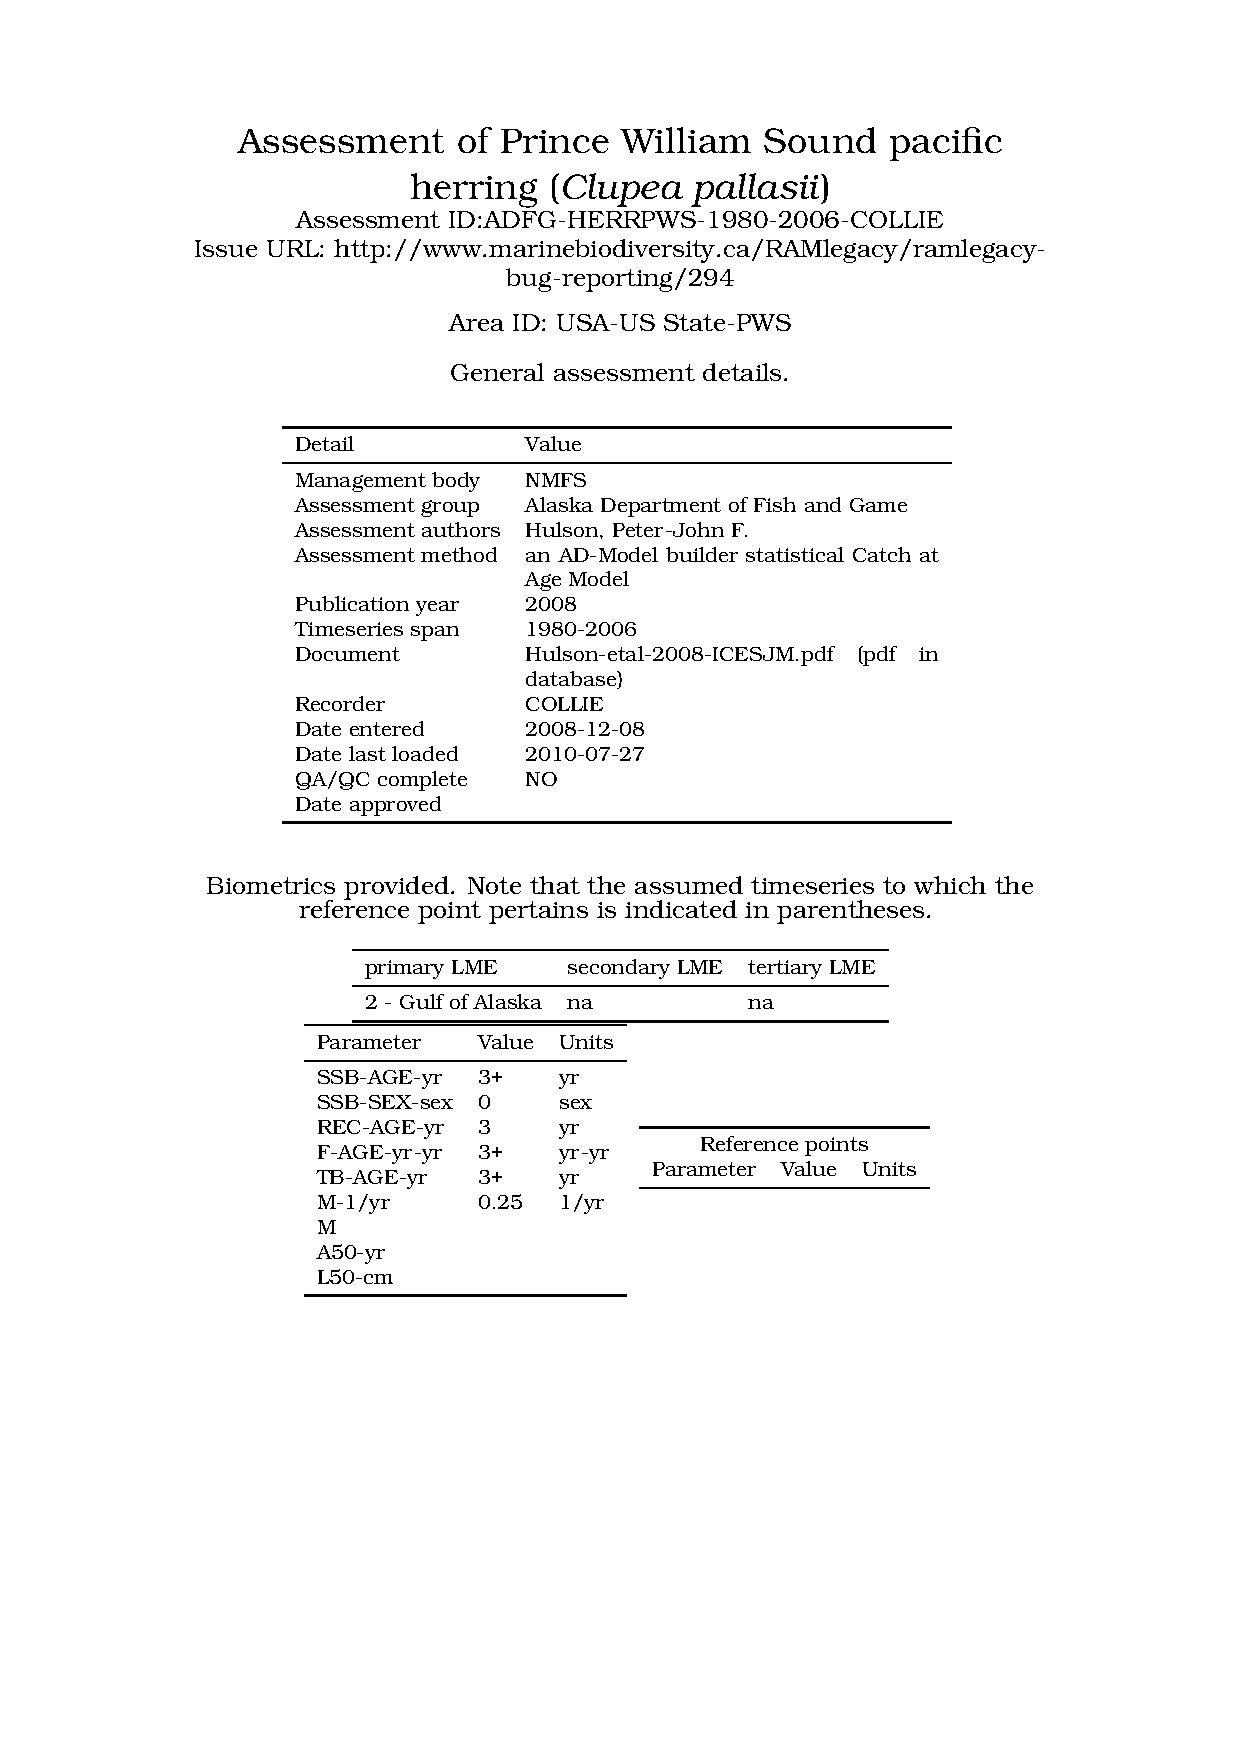
\includepdf[pagecommand={\thispagestyle{plain}}, addtotoc={1,subsubsection,1,ADFG-HERRPWS-1980-2006-COLLIE,ADFG-HERRPWS-1980-2006-COLLIE}, pages={1,2}]{/home/srdbadmin/SQLpg/srdb/trunk/tex/ADFG-HERRPWS-1980-2006-COLLIE.pdf}
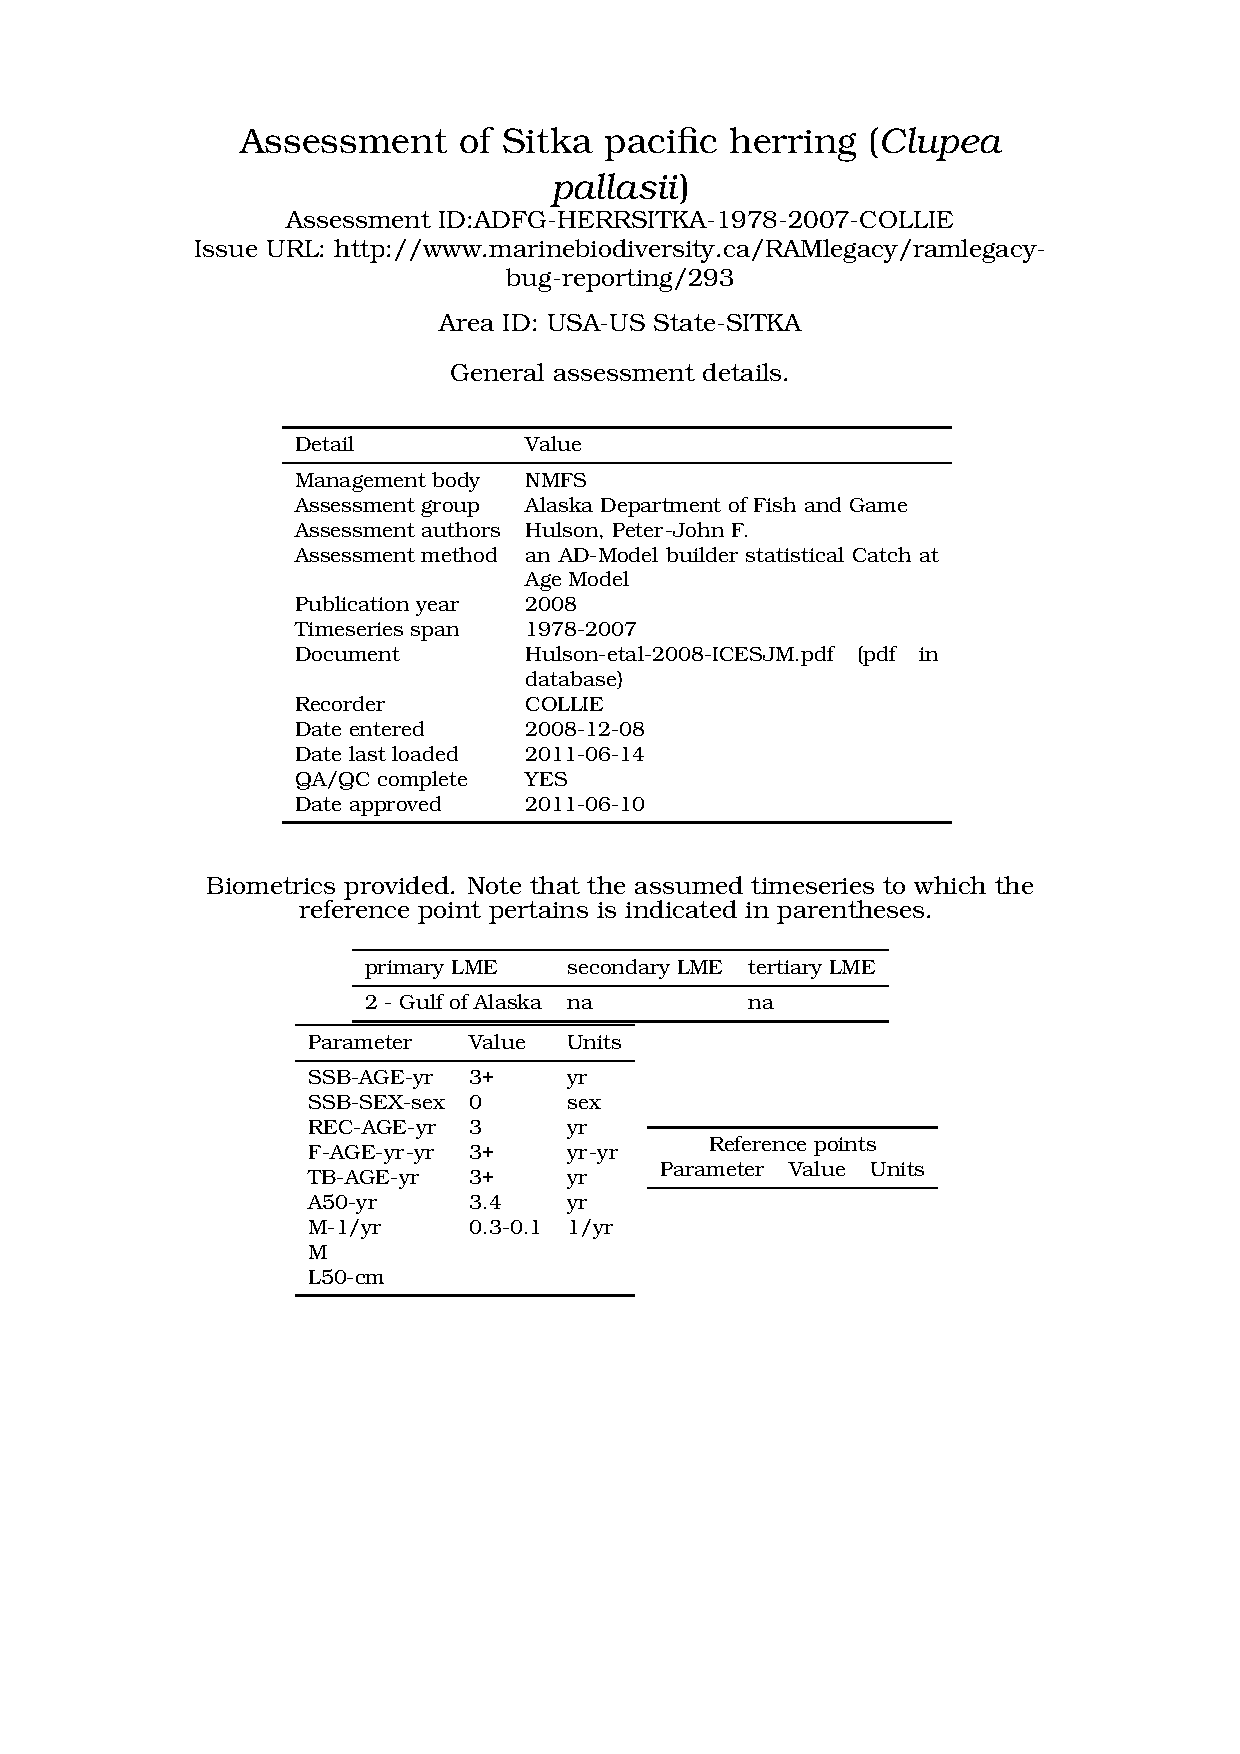
\includepdf[pagecommand={\thispagestyle{plain}}, addtotoc={1,subsubsection,1,ADFG-HERRSITKA-1978-2007-COLLIE,ADFG-HERRSITKA-1978-2007-COLLIE}, pages={1,2}]{/home/srdbadmin/SQLpg/srdb/trunk/tex/ADFG-HERRSITKA-1978-2007-COLLIE.pdf}
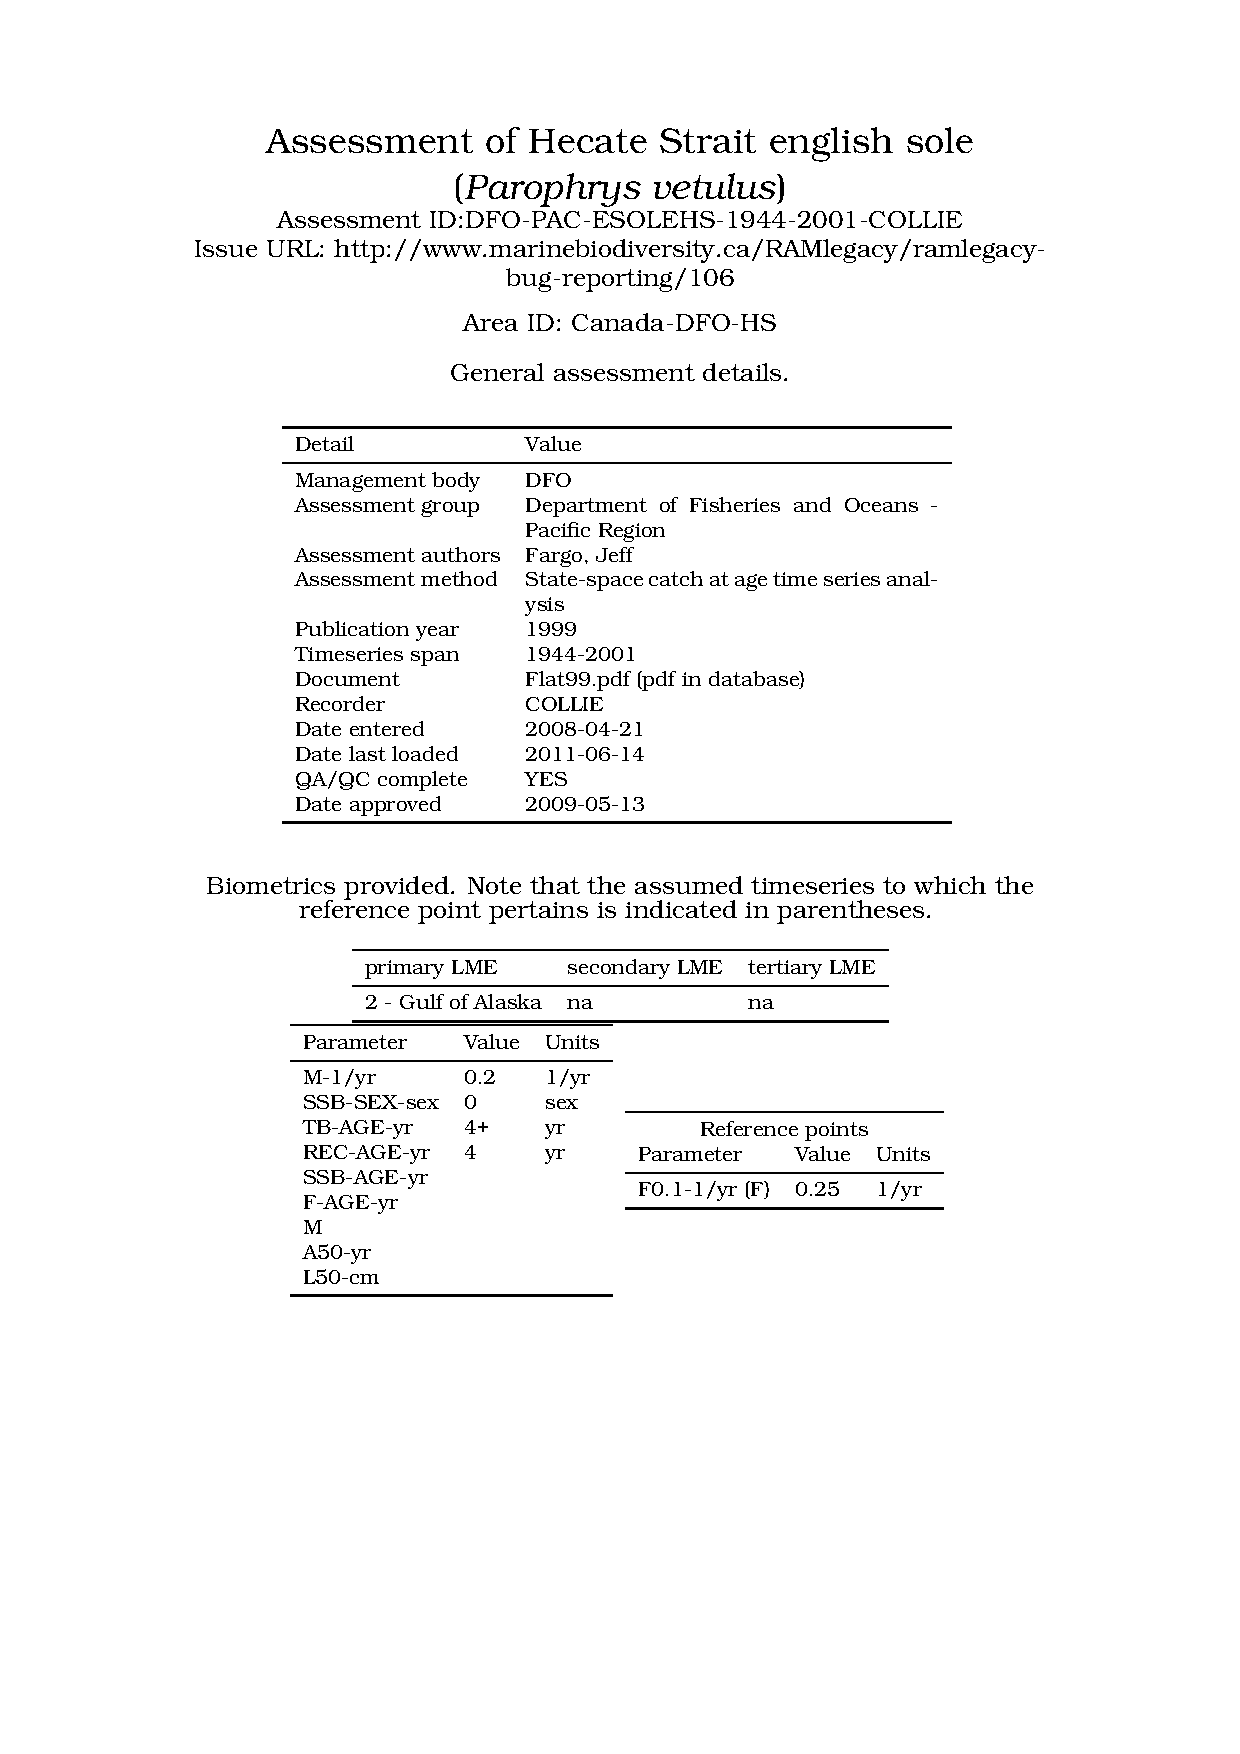
\includepdf[pagecommand={\thispagestyle{plain}}, addtotoc={1,subsubsection,1,DFO-PAC-ESOLEHS-1944-2001-COLLIE,DFO-PAC-ESOLEHS-1944-2001-COLLIE}, pages={1,2}]{/home/srdbadmin/SQLpg/srdb/trunk/tex/DFO-PAC-ESOLEHS-1944-2001-COLLIE.pdf}
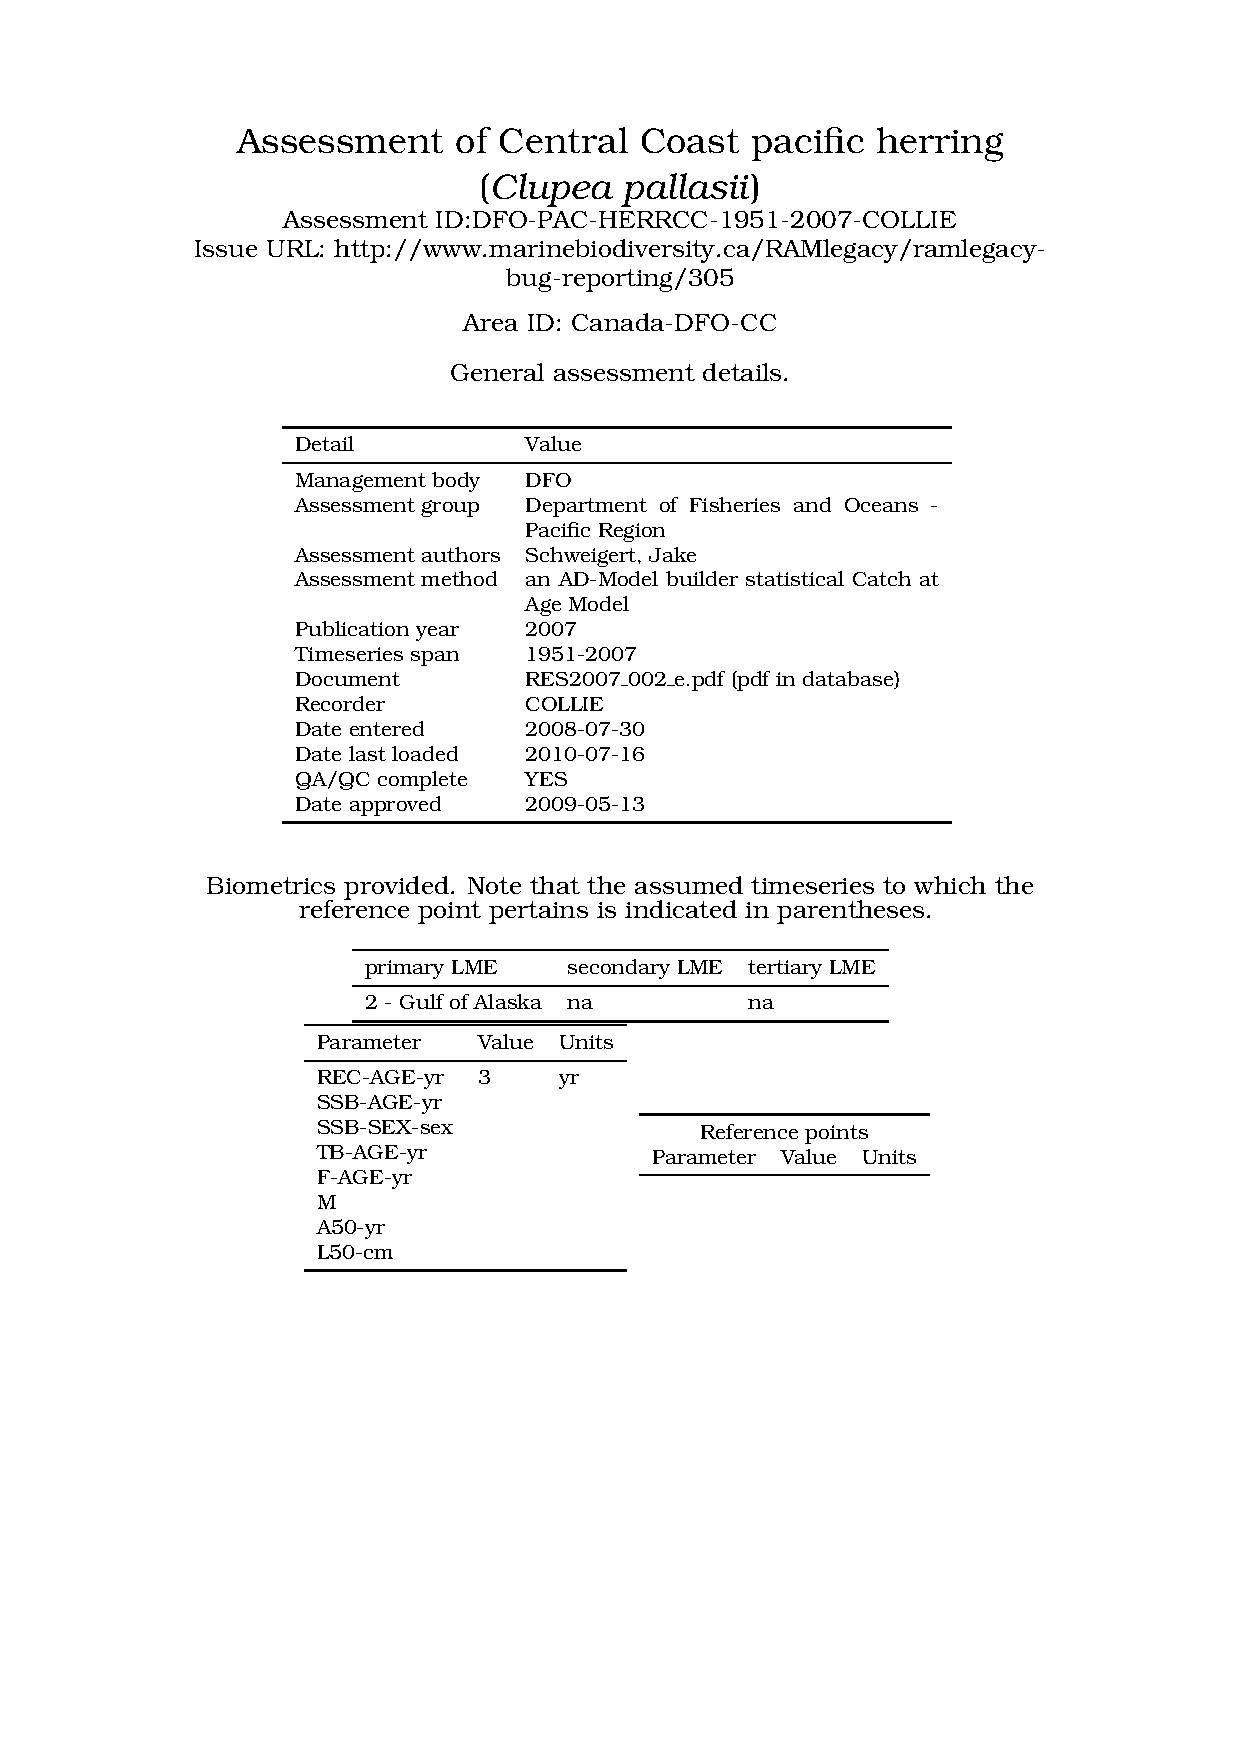
\includepdf[pagecommand={\thispagestyle{plain}}, addtotoc={1,subsubsection,1,DFO-PAC-HERRCC-1951-2007-COLLIE,DFO-PAC-HERRCC-1951-2007-COLLIE}, pages={1,2}]{/home/srdbadmin/SQLpg/srdb/trunk/tex/DFO-PAC-HERRCC-1951-2007-COLLIE.pdf}
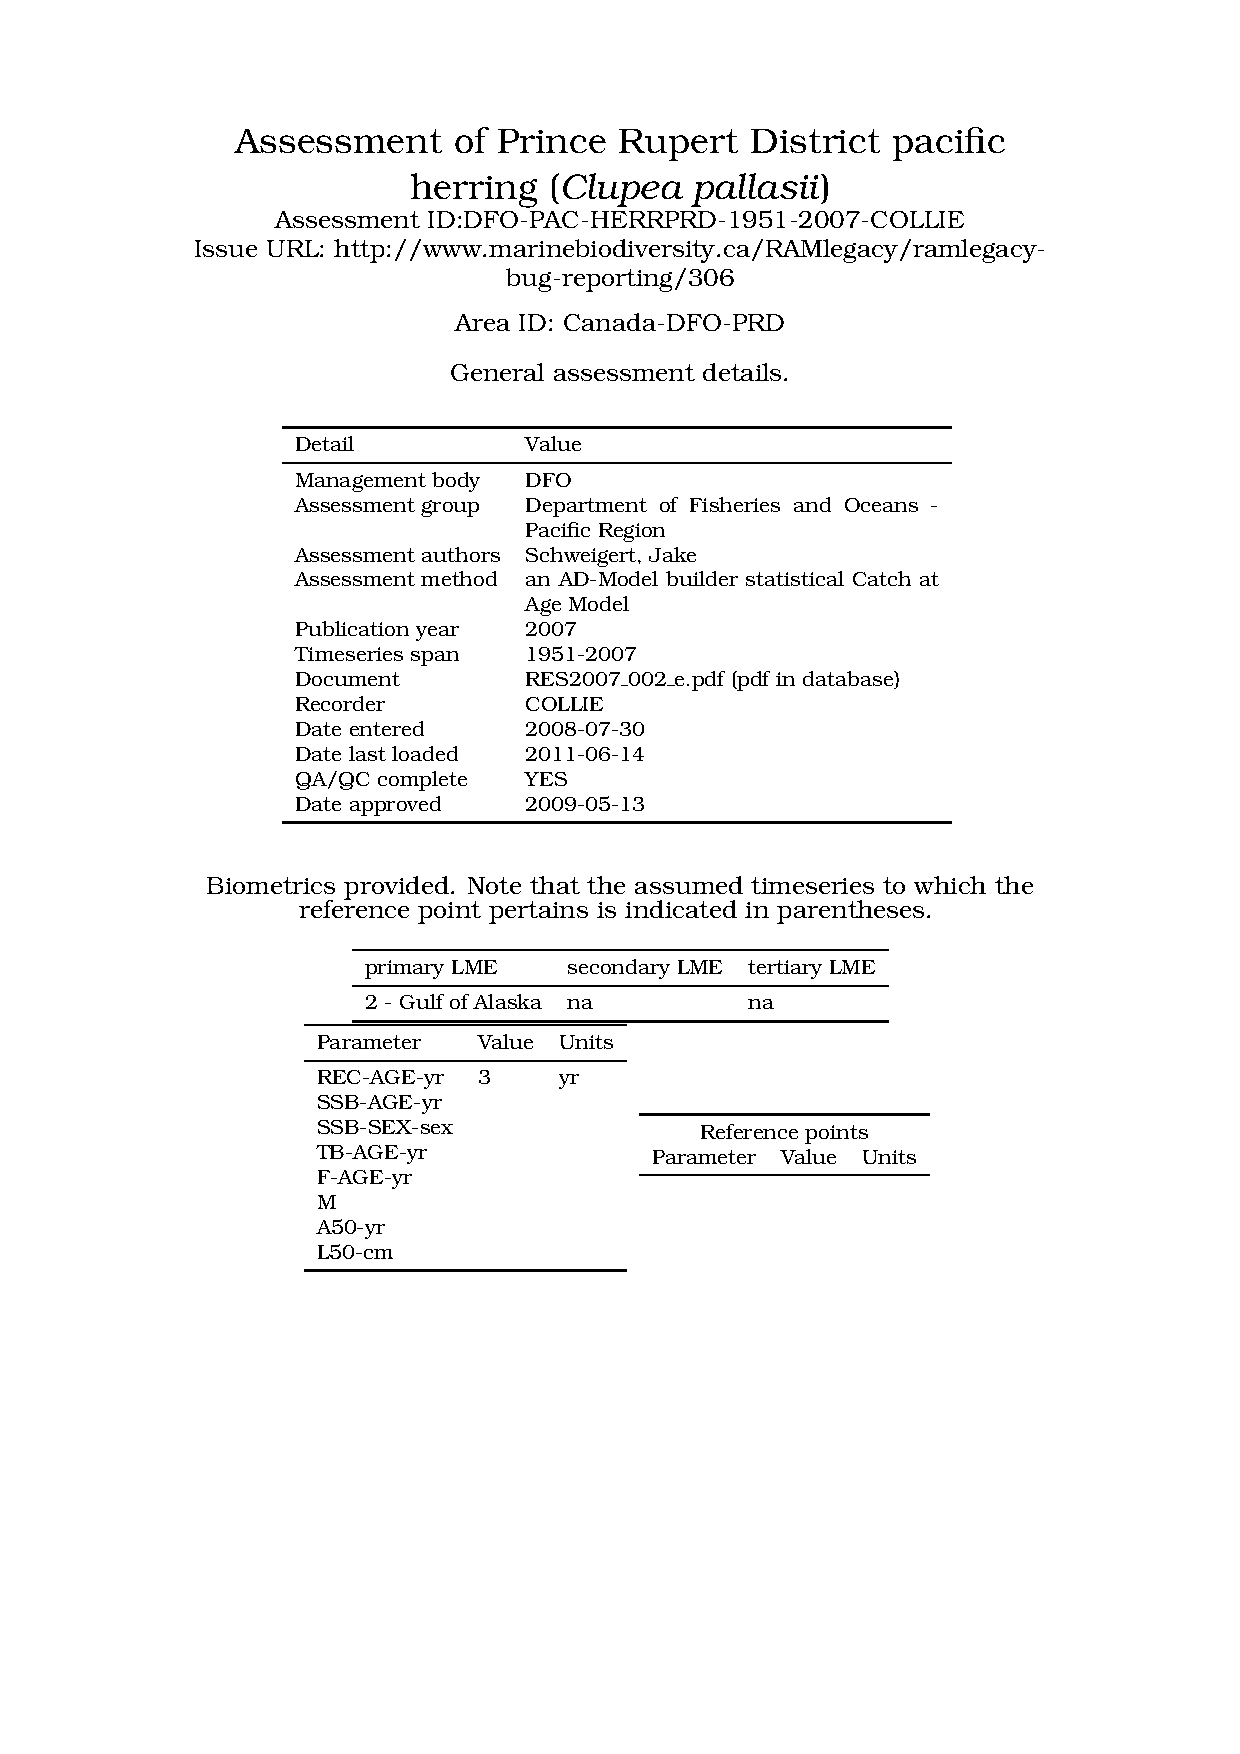
\includepdf[pagecommand={\thispagestyle{plain}}, addtotoc={1,subsubsection,1,DFO-PAC-HERRPRD-1951-2007-COLLIE,DFO-PAC-HERRPRD-1951-2007-COLLIE}, pages={1,2}]{/home/srdbadmin/SQLpg/srdb/trunk/tex/DFO-PAC-HERRPRD-1951-2007-COLLIE.pdf}
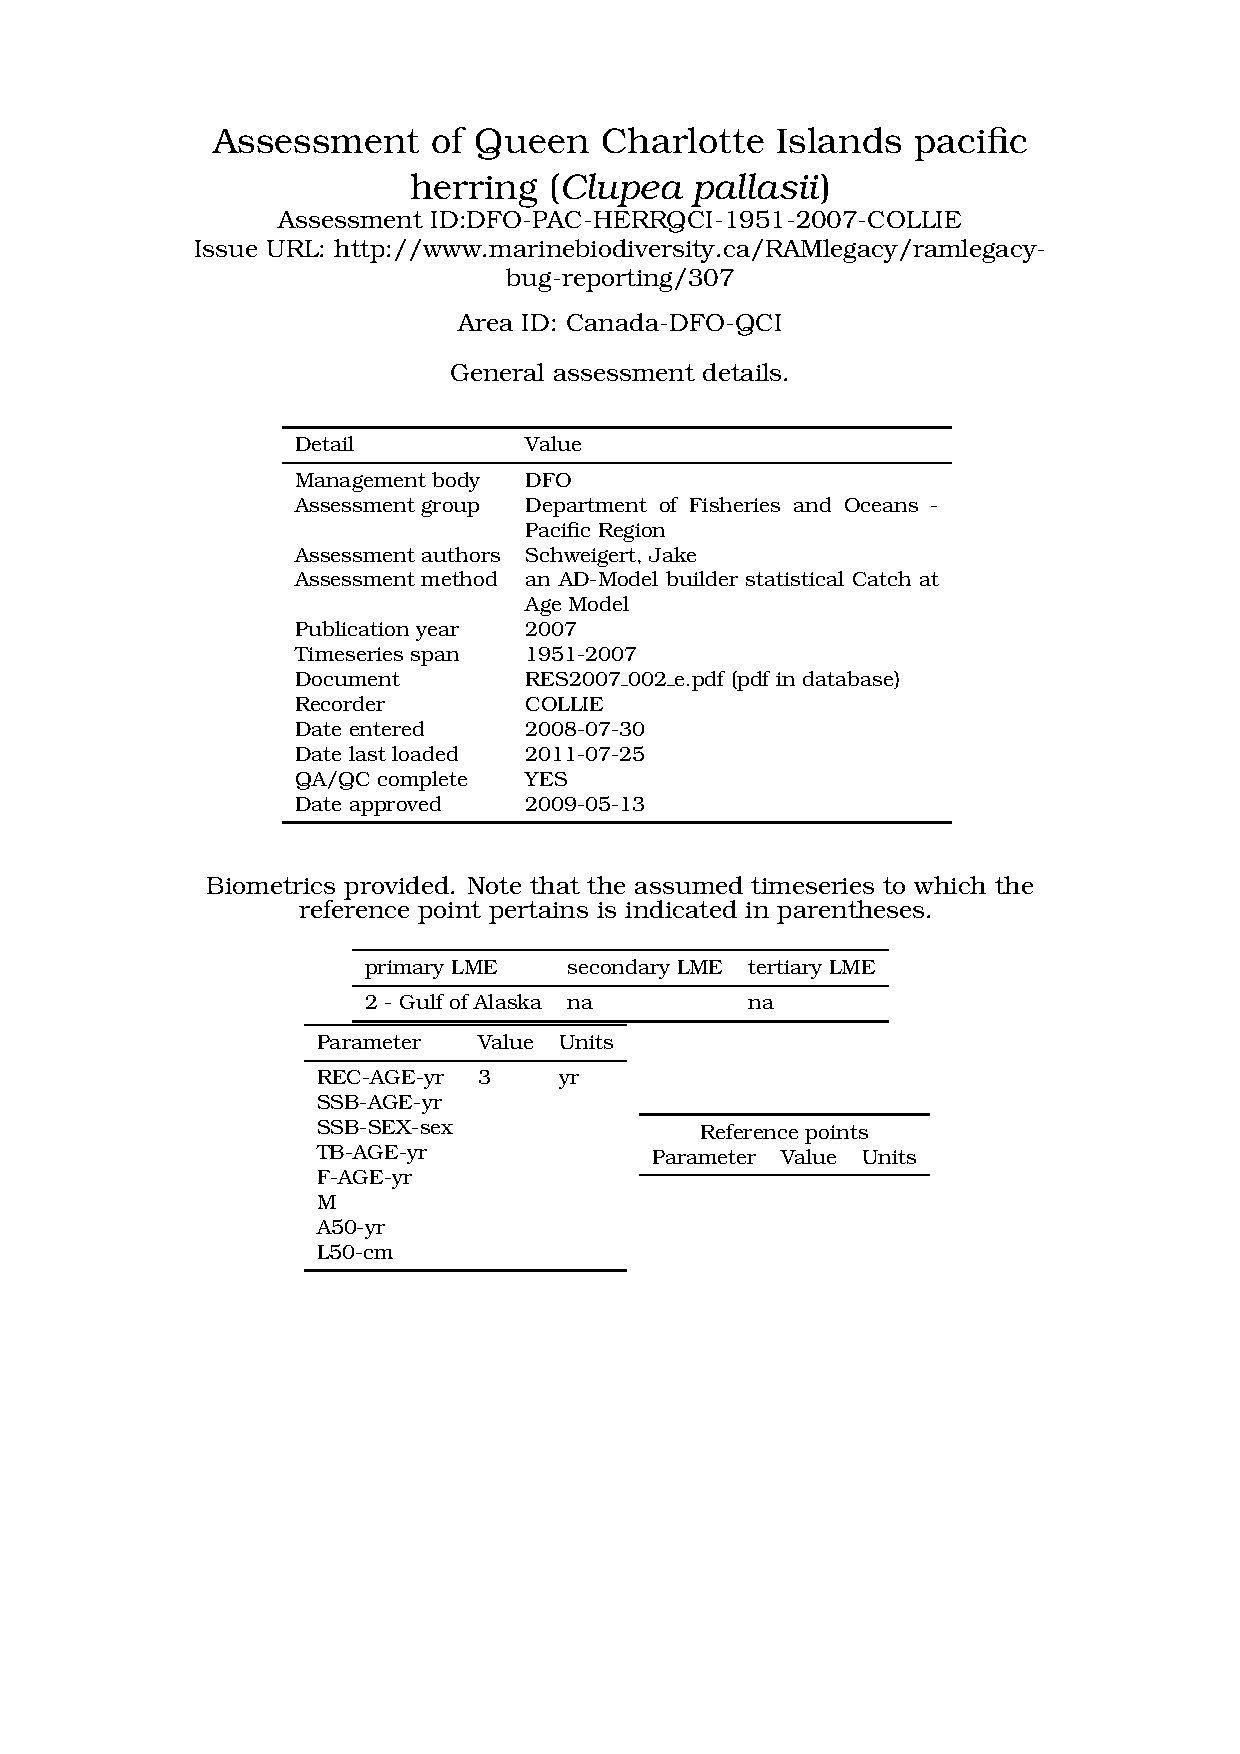
\includepdf[pagecommand={\thispagestyle{plain}}, addtotoc={1,subsubsection,1,DFO-PAC-HERRQCI-1951-2007-COLLIE,DFO-PAC-HERRQCI-1951-2007-COLLIE}, pages={1,2}]{/home/srdbadmin/SQLpg/srdb/trunk/tex/DFO-PAC-HERRQCI-1951-2007-COLLIE.pdf}
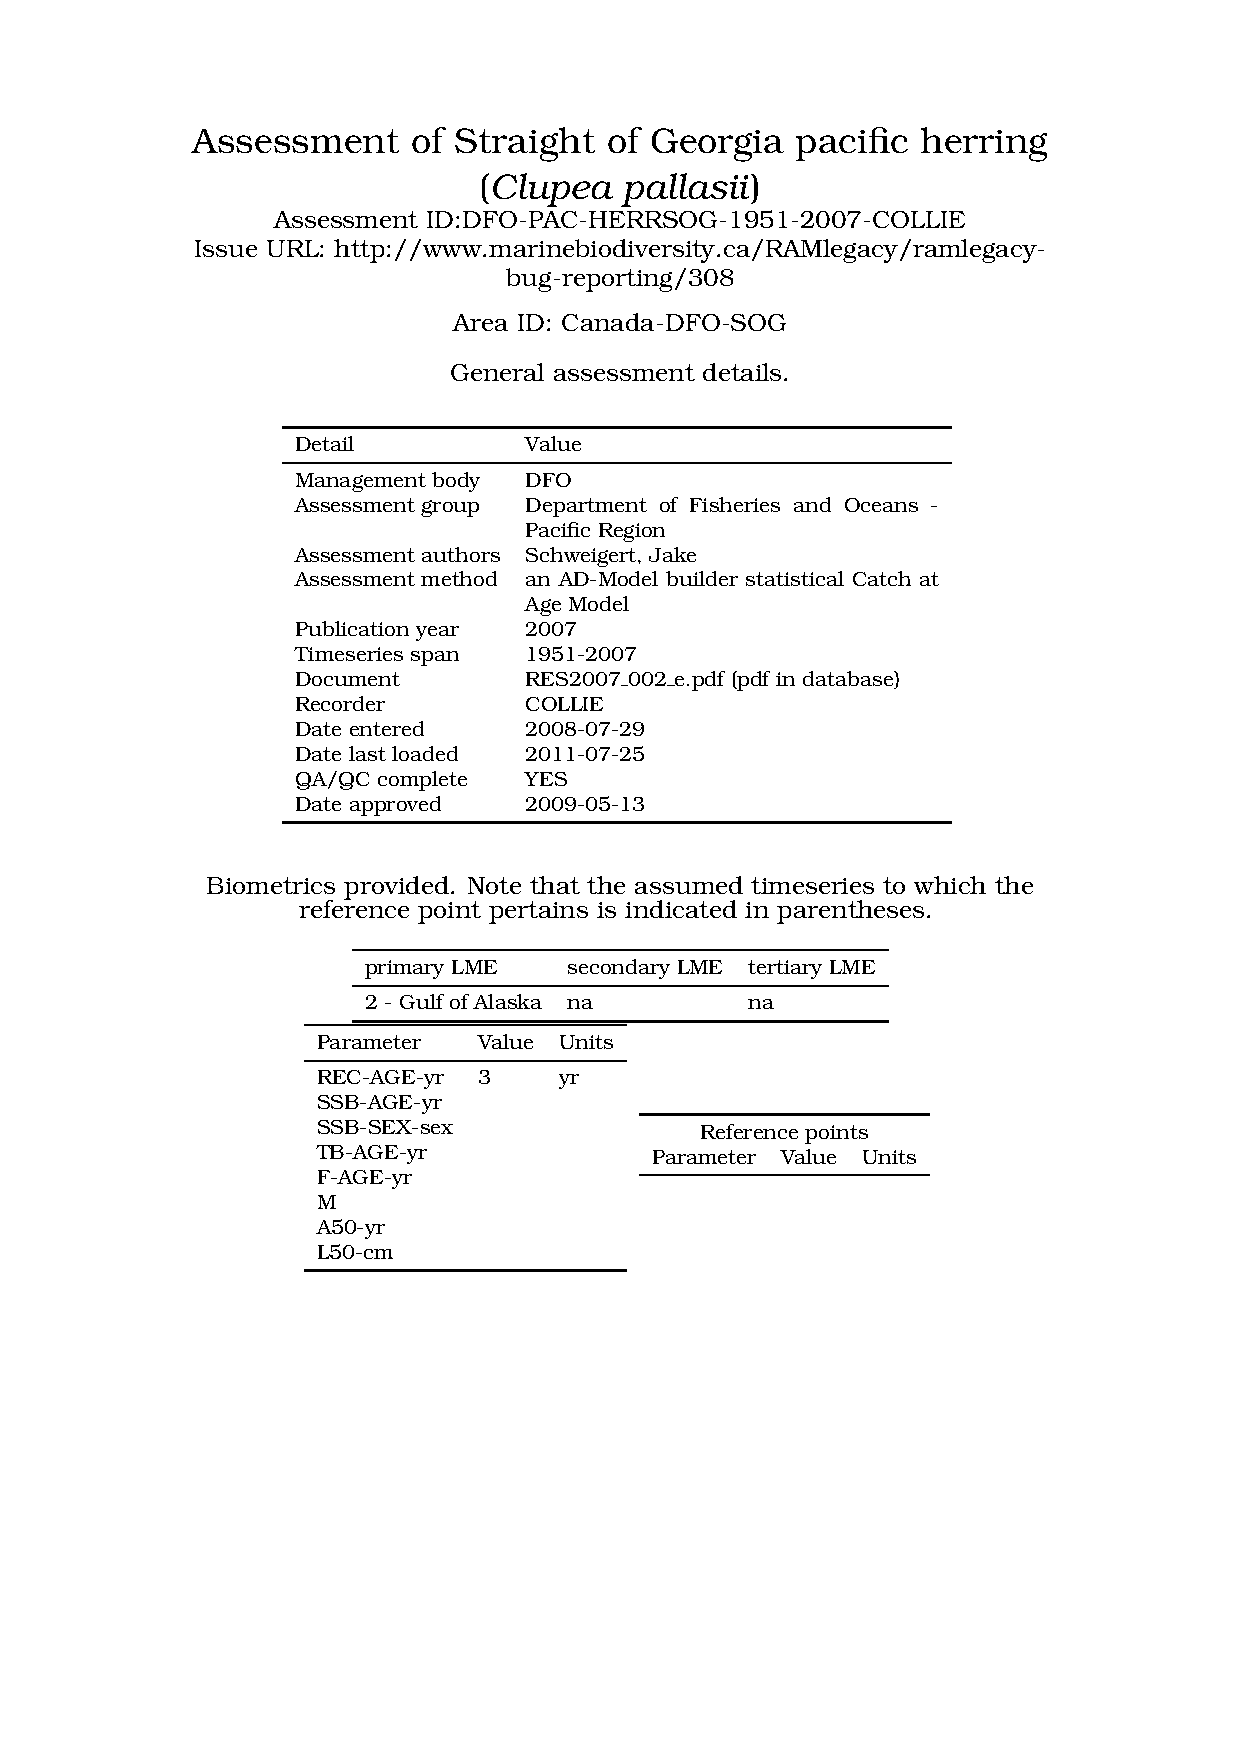
\includepdf[pagecommand={\thispagestyle{plain}}, addtotoc={1,subsubsection,1,DFO-PAC-HERRSOG-1951-2007-COLLIE,DFO-PAC-HERRSOG-1951-2007-COLLIE}, pages={1,2}]{/home/srdbadmin/SQLpg/srdb/trunk/tex/DFO-PAC-HERRSOG-1951-2007-COLLIE.pdf}
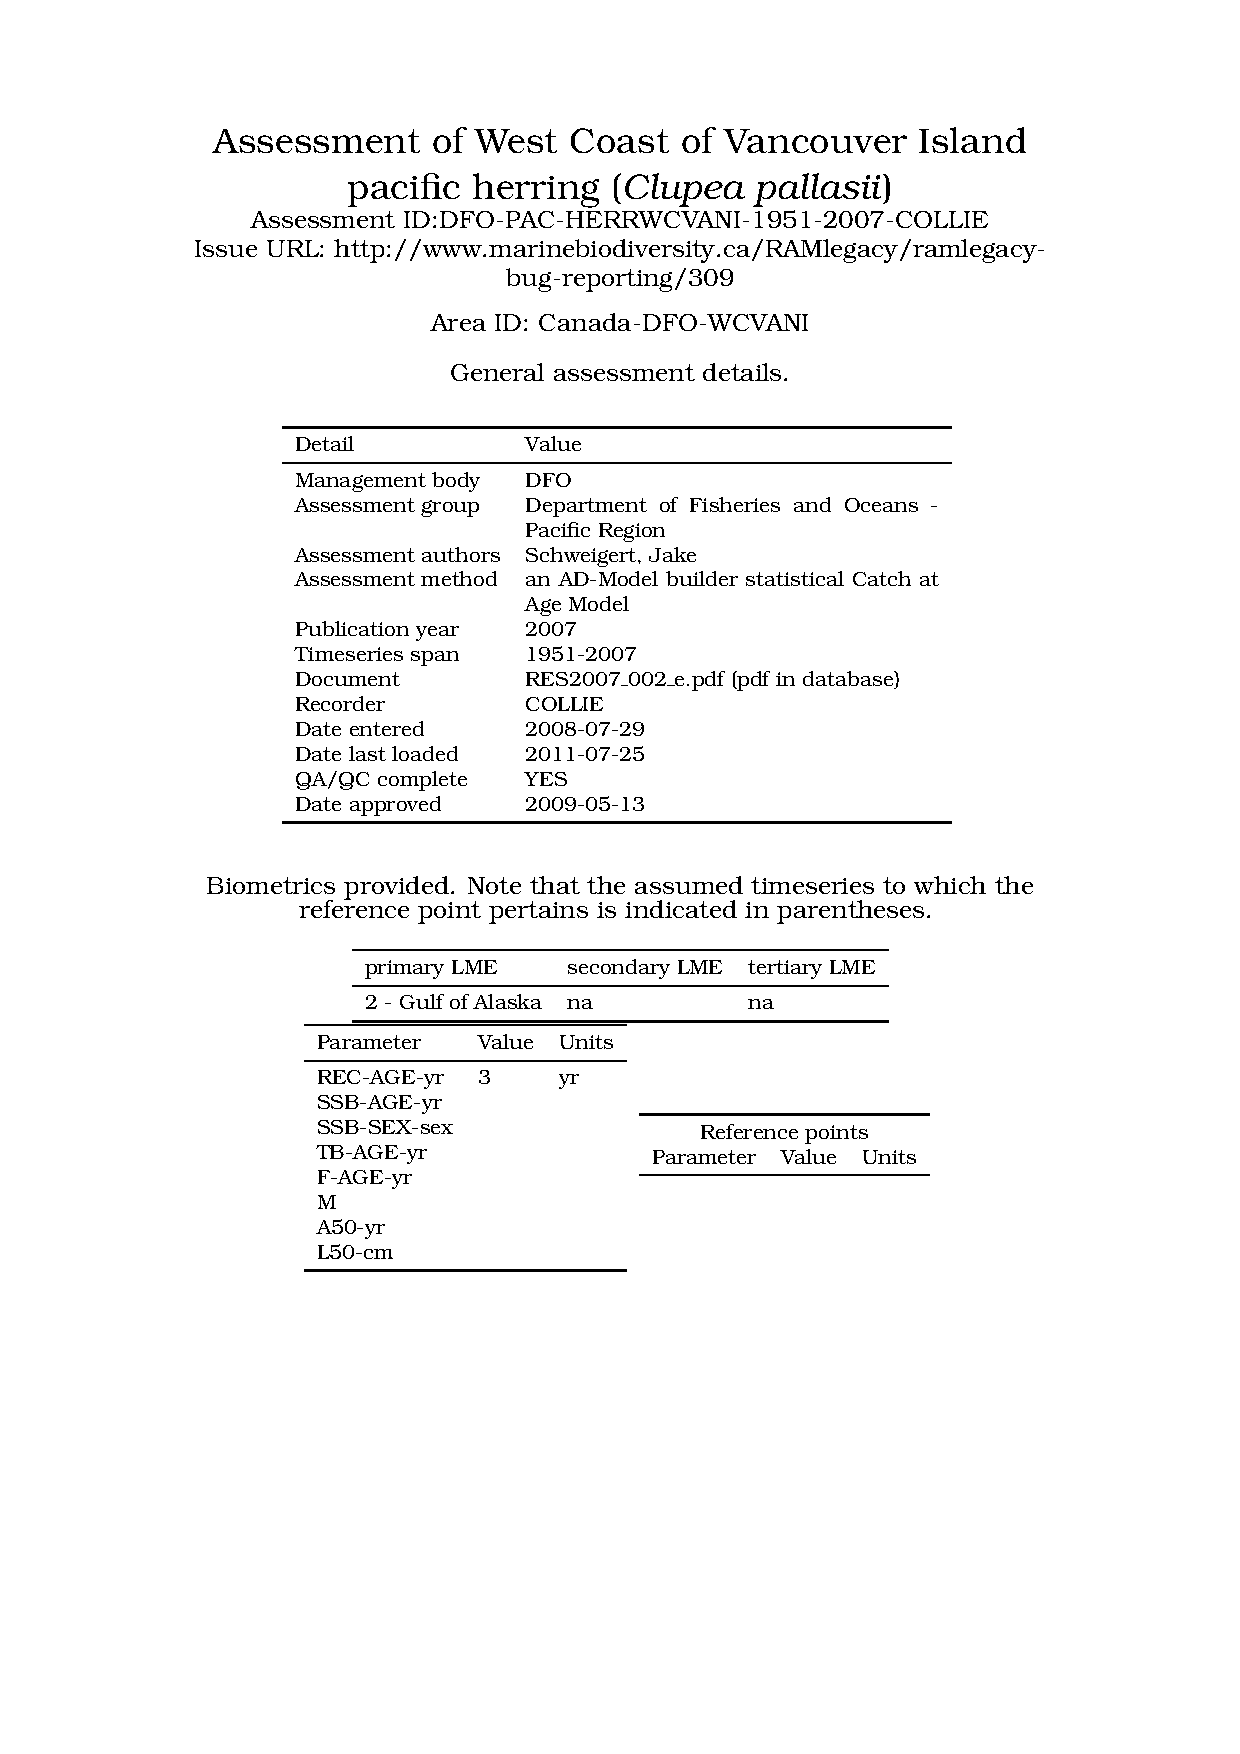
\includepdf[pagecommand={\thispagestyle{plain}}, addtotoc={1,subsubsection,1,DFO-PAC-HERRWCVANI-1951-2007-COLLIE,DFO-PAC-HERRWCVANI-1951-2007-COLLIE}, pages={1,2}]{/home/srdbadmin/SQLpg/srdb/trunk/tex/DFO-PAC-HERRWCVANI-1951-2007-COLLIE.pdf}
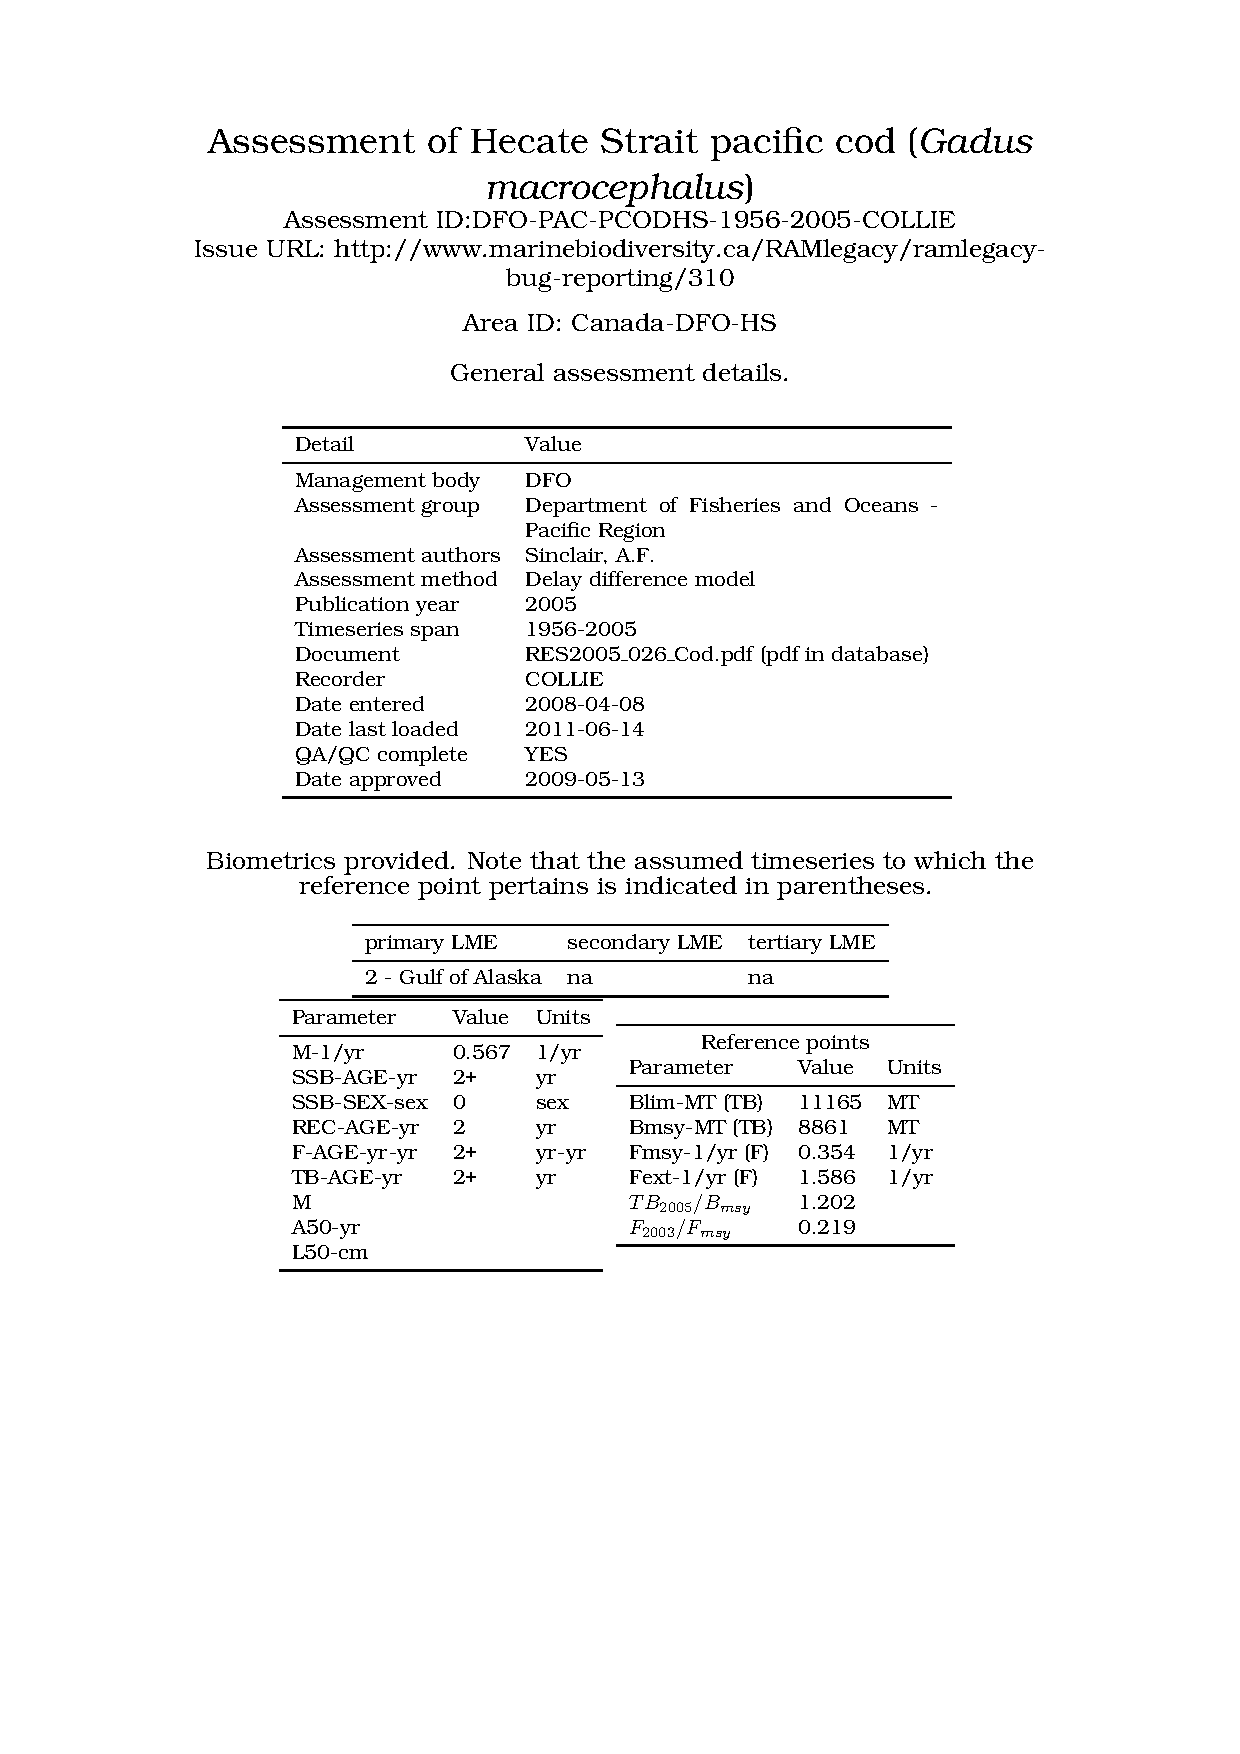
\includepdf[pagecommand={\thispagestyle{plain}}, addtotoc={1,subsubsection,1,DFO-PAC-PCODHS-1956-2005-COLLIE,DFO-PAC-PCODHS-1956-2005-COLLIE}, pages={1,2}]{/home/srdbadmin/SQLpg/srdb/trunk/tex/DFO-PAC-PCODHS-1956-2005-COLLIE.pdf}
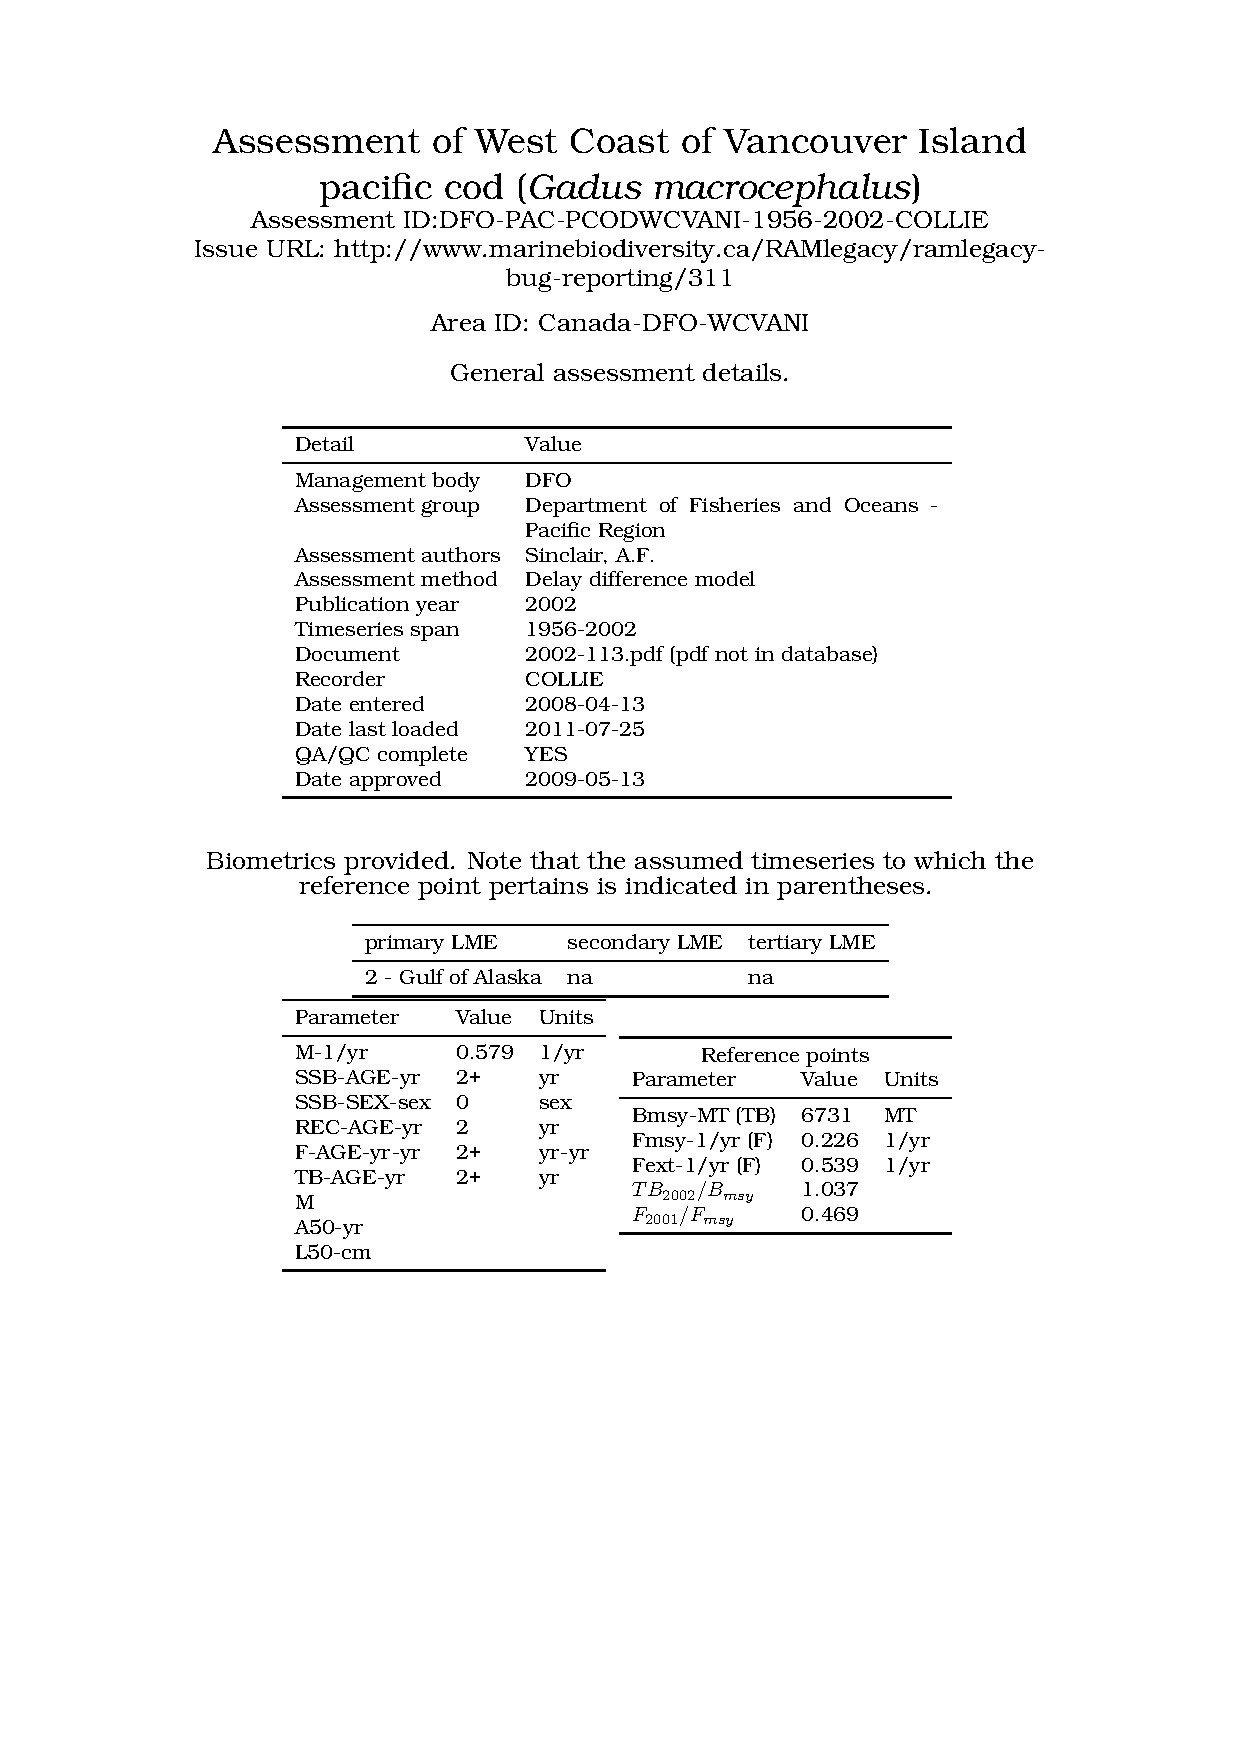
\includepdf[pagecommand={\thispagestyle{plain}}, addtotoc={1,subsubsection,1,DFO-PAC-PCODWCVANI-1956-2002-COLLIE,DFO-PAC-PCODWCVANI-1956-2002-COLLIE}, pages={1,2}]{/home/srdbadmin/SQLpg/srdb/trunk/tex/DFO-PAC-PCODWCVANI-1956-2002-COLLIE.pdf}
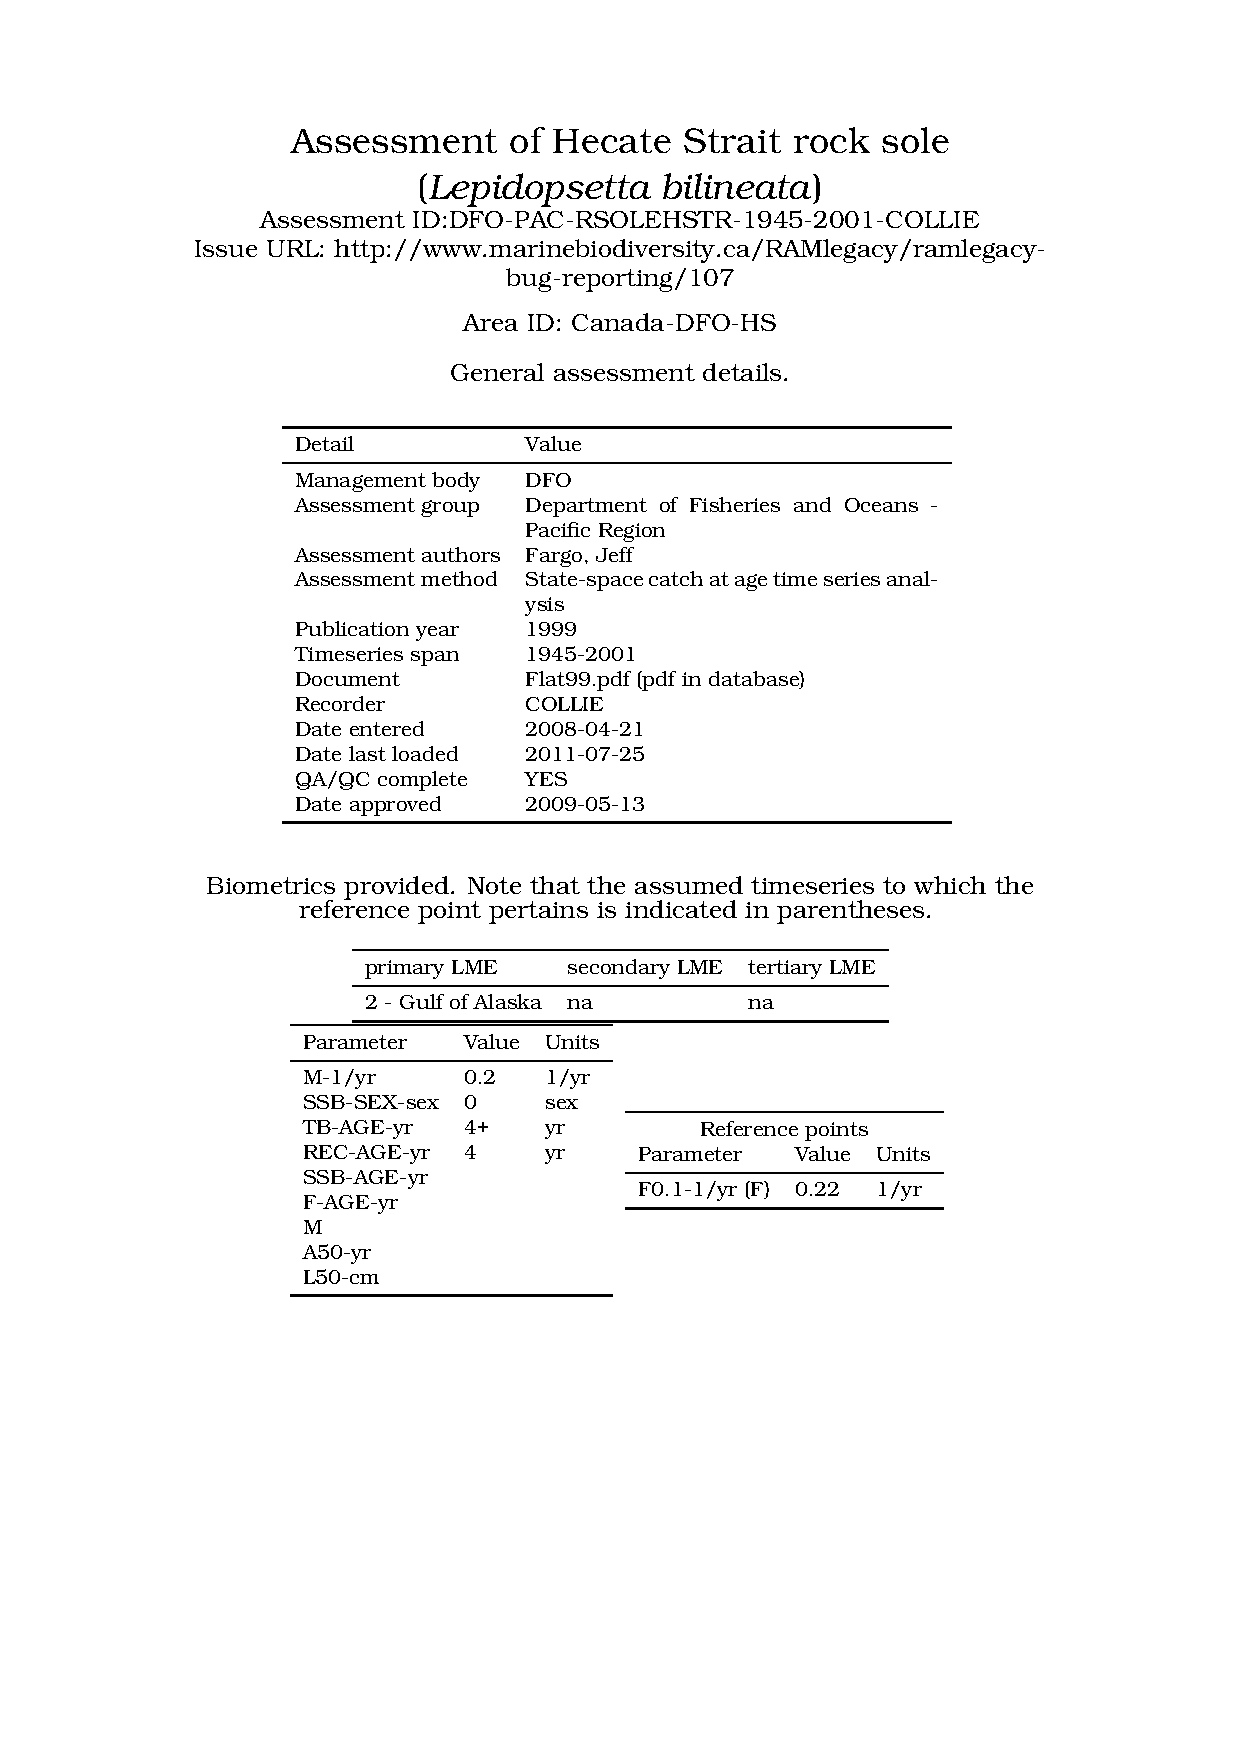
\includepdf[pagecommand={\thispagestyle{plain}}, addtotoc={1,subsubsection,1,DFO-PAC-RSOLEHSTR-1945-2001-COLLIE,DFO-PAC-RSOLEHSTR-1945-2001-COLLIE}, pages={1,2}]{/home/srdbadmin/SQLpg/srdb/trunk/tex/DFO-PAC-RSOLEHSTR-1945-2001-COLLIE.pdf}
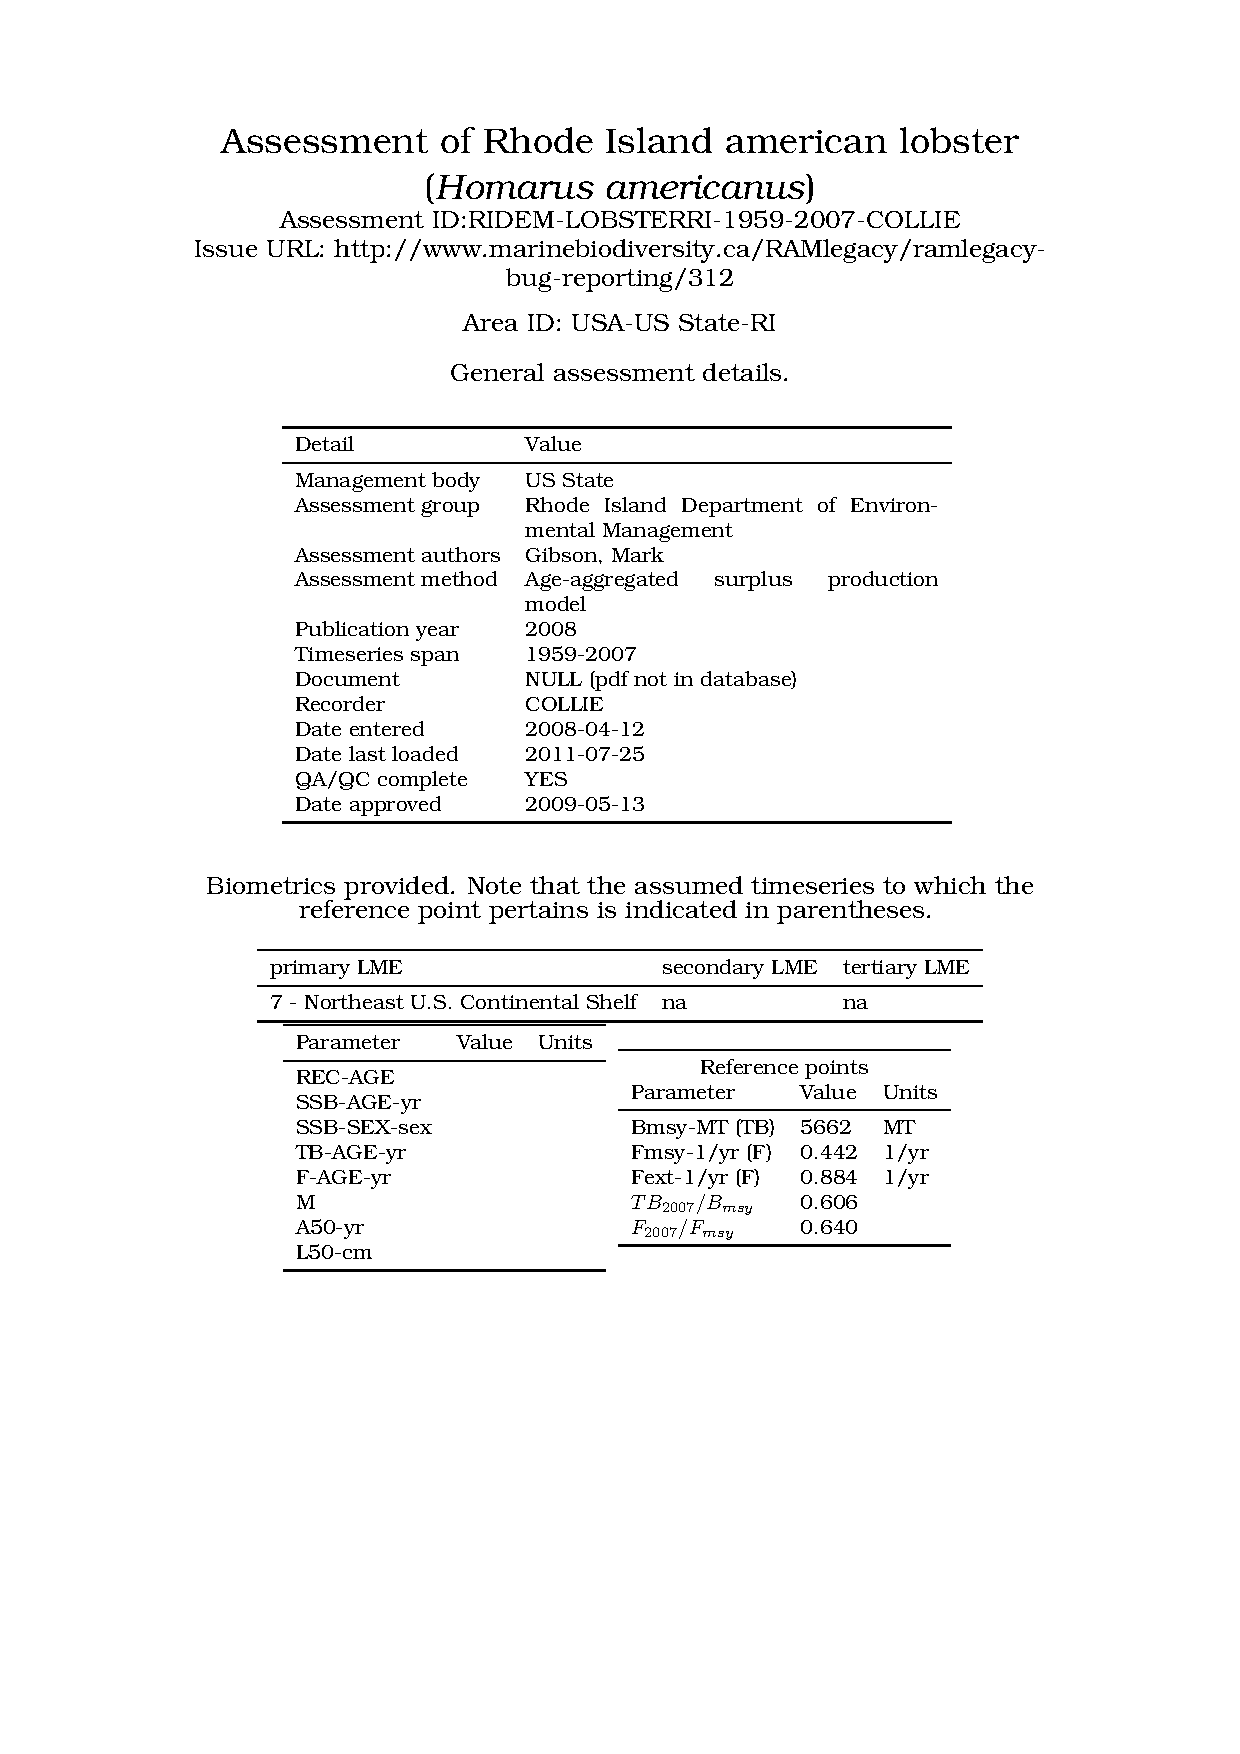
\includepdf[pagecommand={\thispagestyle{plain}}, addtotoc={1,subsubsection,1,RIDEM-LOBSTERRI-1959-2007-COLLIE,RIDEM-LOBSTERRI-1959-2007-COLLIE}, pages={1,2}]{/home/srdbadmin/SQLpg/srdb/trunk/tex/RIDEM-LOBSTERRI-1959-2007-COLLIE.pdf}
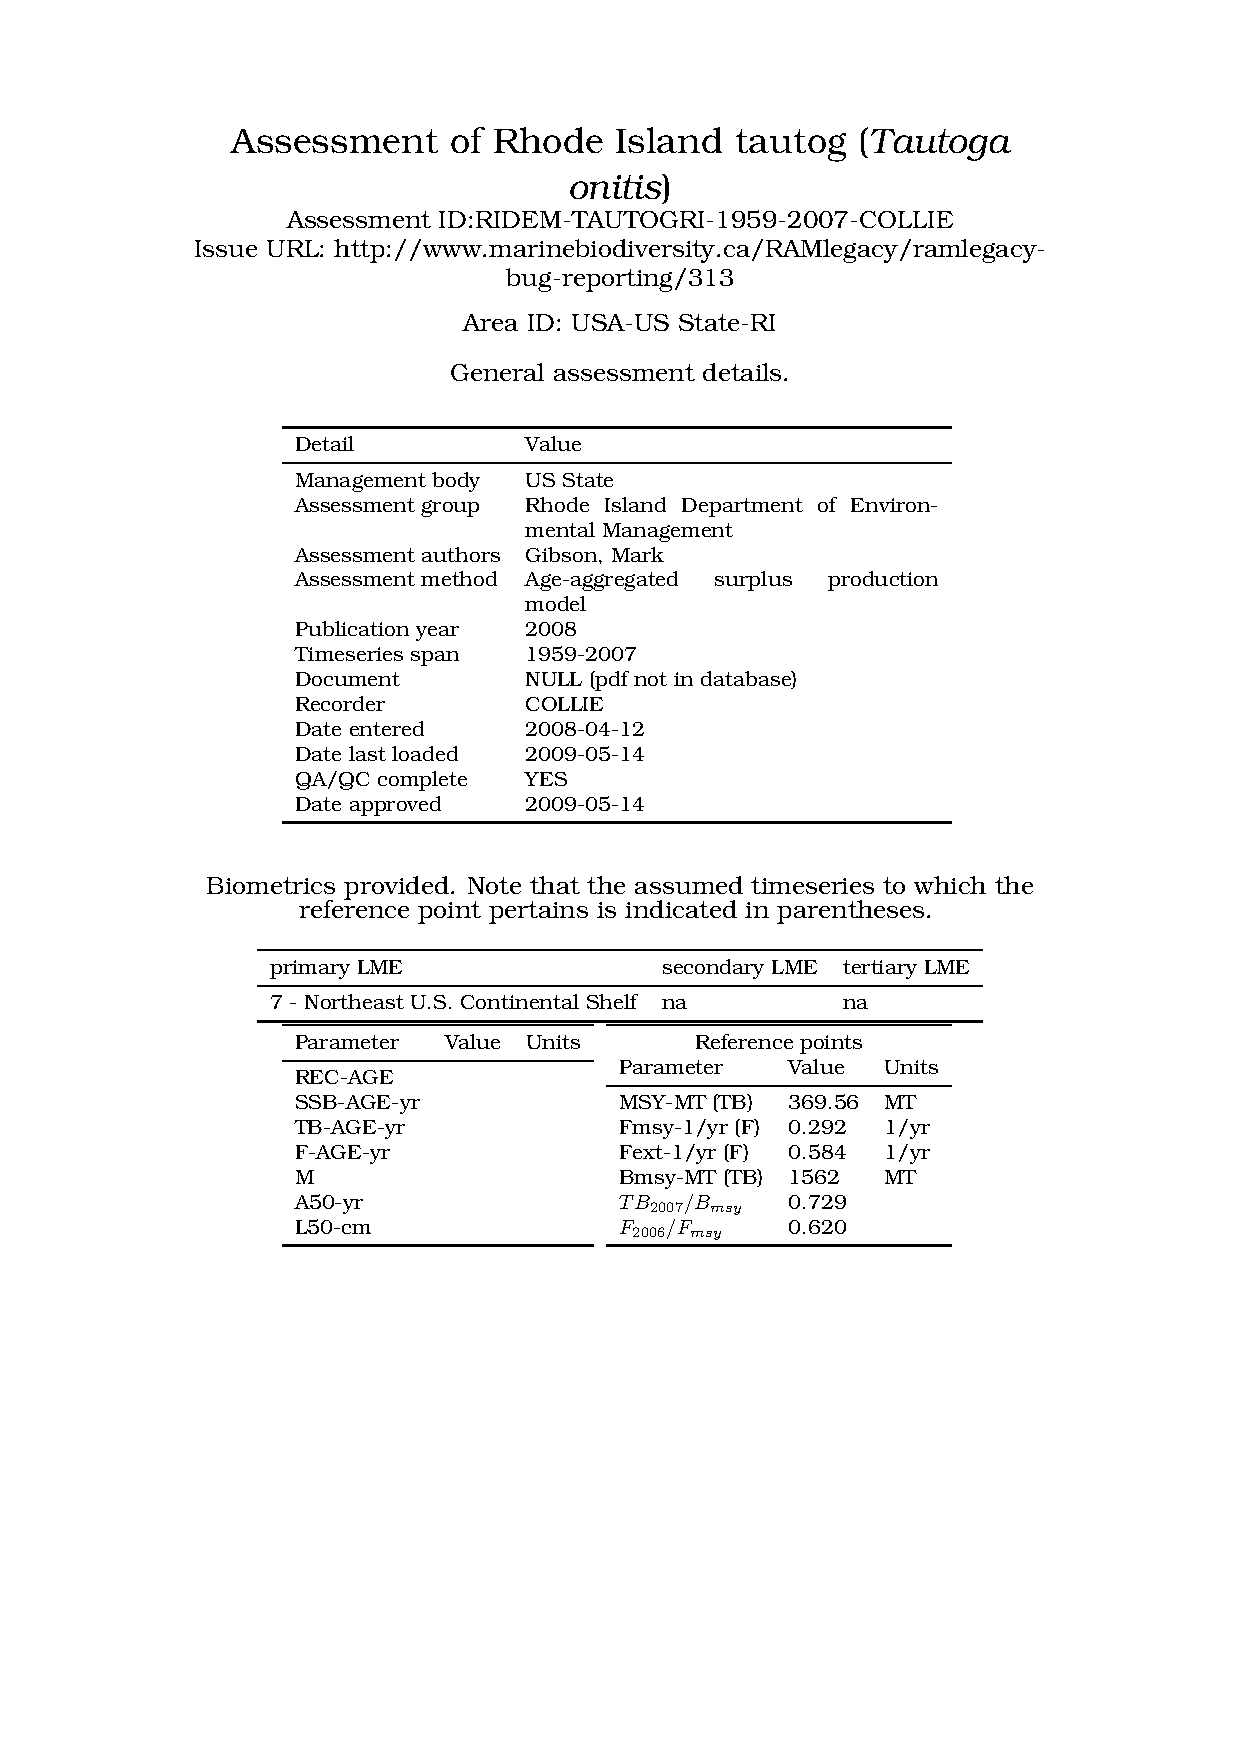
\includepdf[pagecommand={\thispagestyle{plain}}, addtotoc={1,subsubsection,1,RIDEM-TAUTOGRI-1959-2007-COLLIE,RIDEM-TAUTOGRI-1959-2007-COLLIE}, pages={1,2}]{/home/srdbadmin/SQLpg/srdb/trunk/tex/RIDEM-TAUTOGRI-1959-2007-COLLIE.pdf}
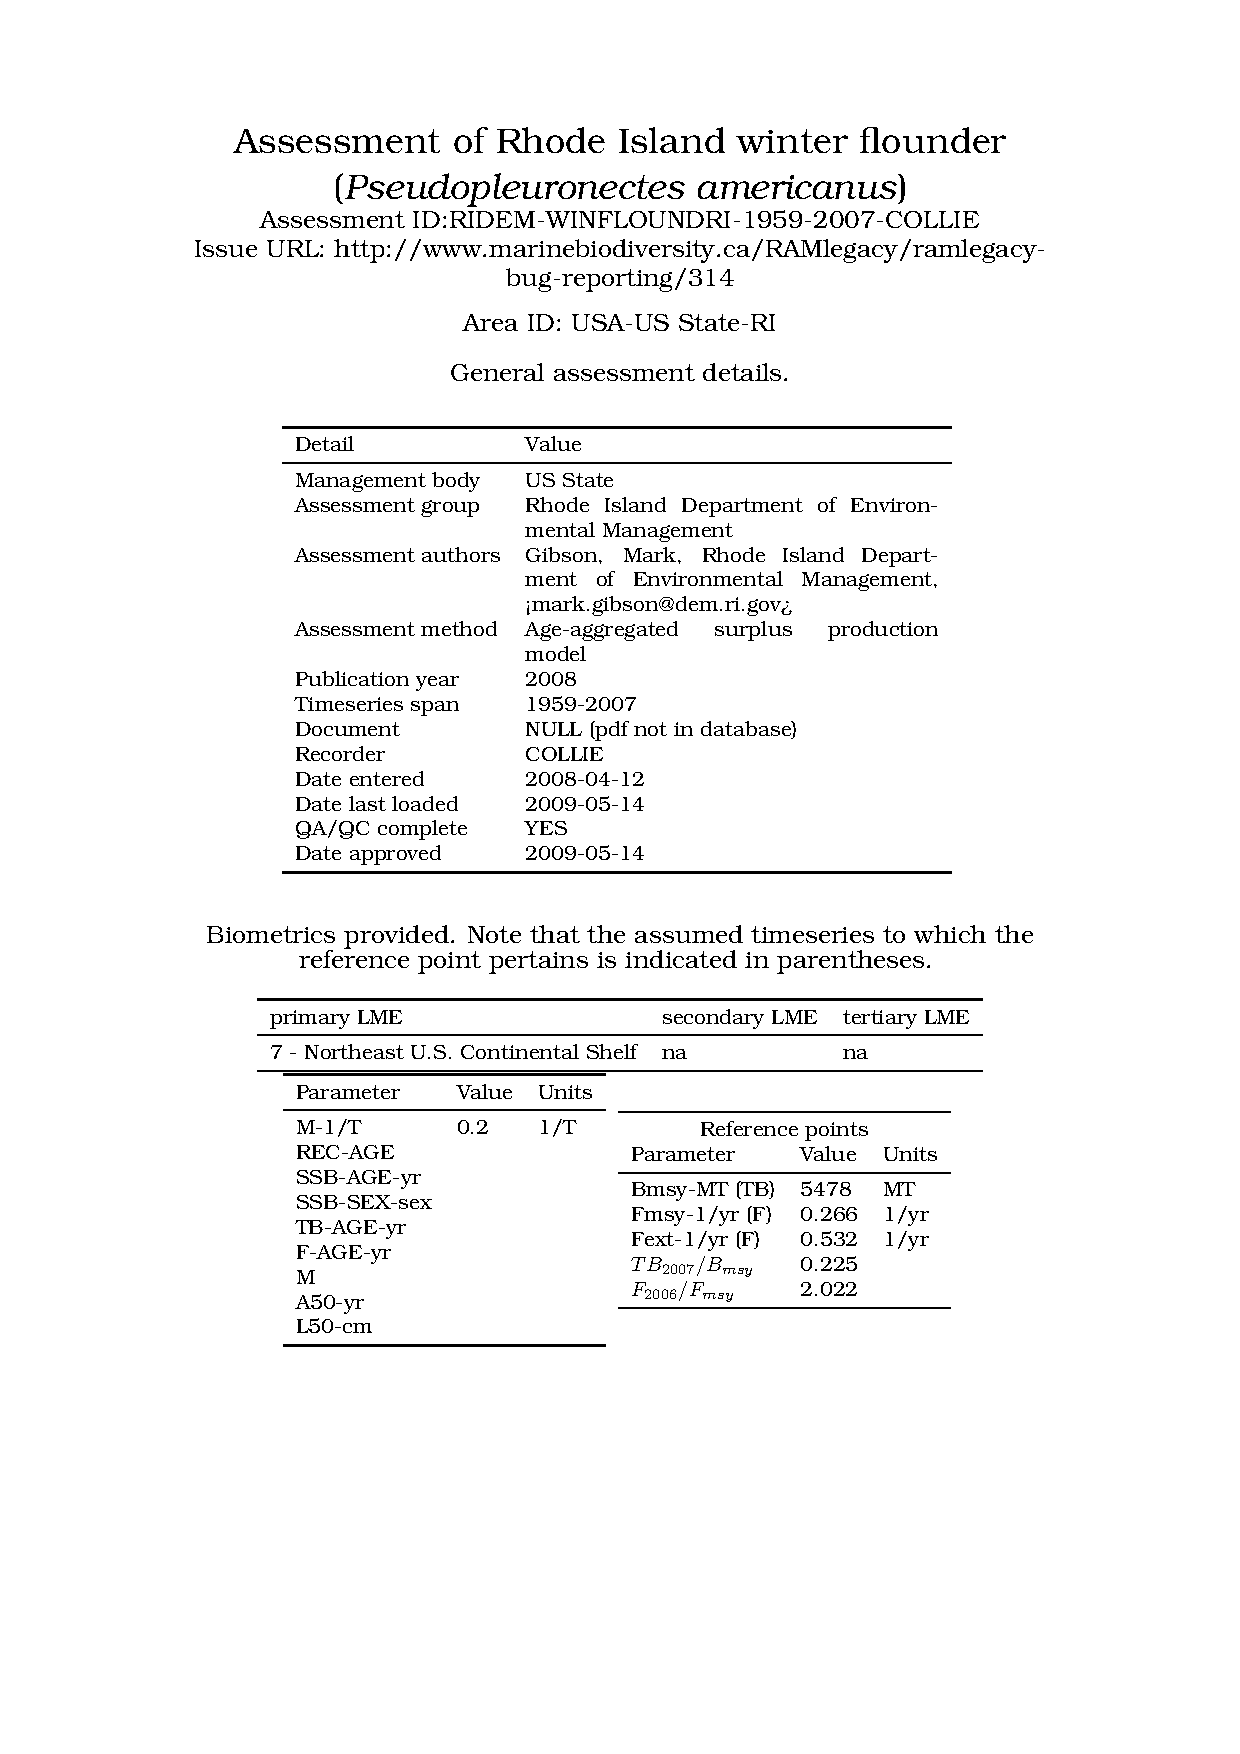
\includepdf[pagecommand={\thispagestyle{plain}}, addtotoc={1,subsubsection,1,RIDEM-WINFLOUNDRI-1959-2007-COLLIE,RIDEM-WINFLOUNDRI-1959-2007-COLLIE}, pages={1,2}]{/home/srdbadmin/SQLpg/srdb/trunk/tex/RIDEM-WINFLOUNDRI-1959-2007-COLLIE.pdf}
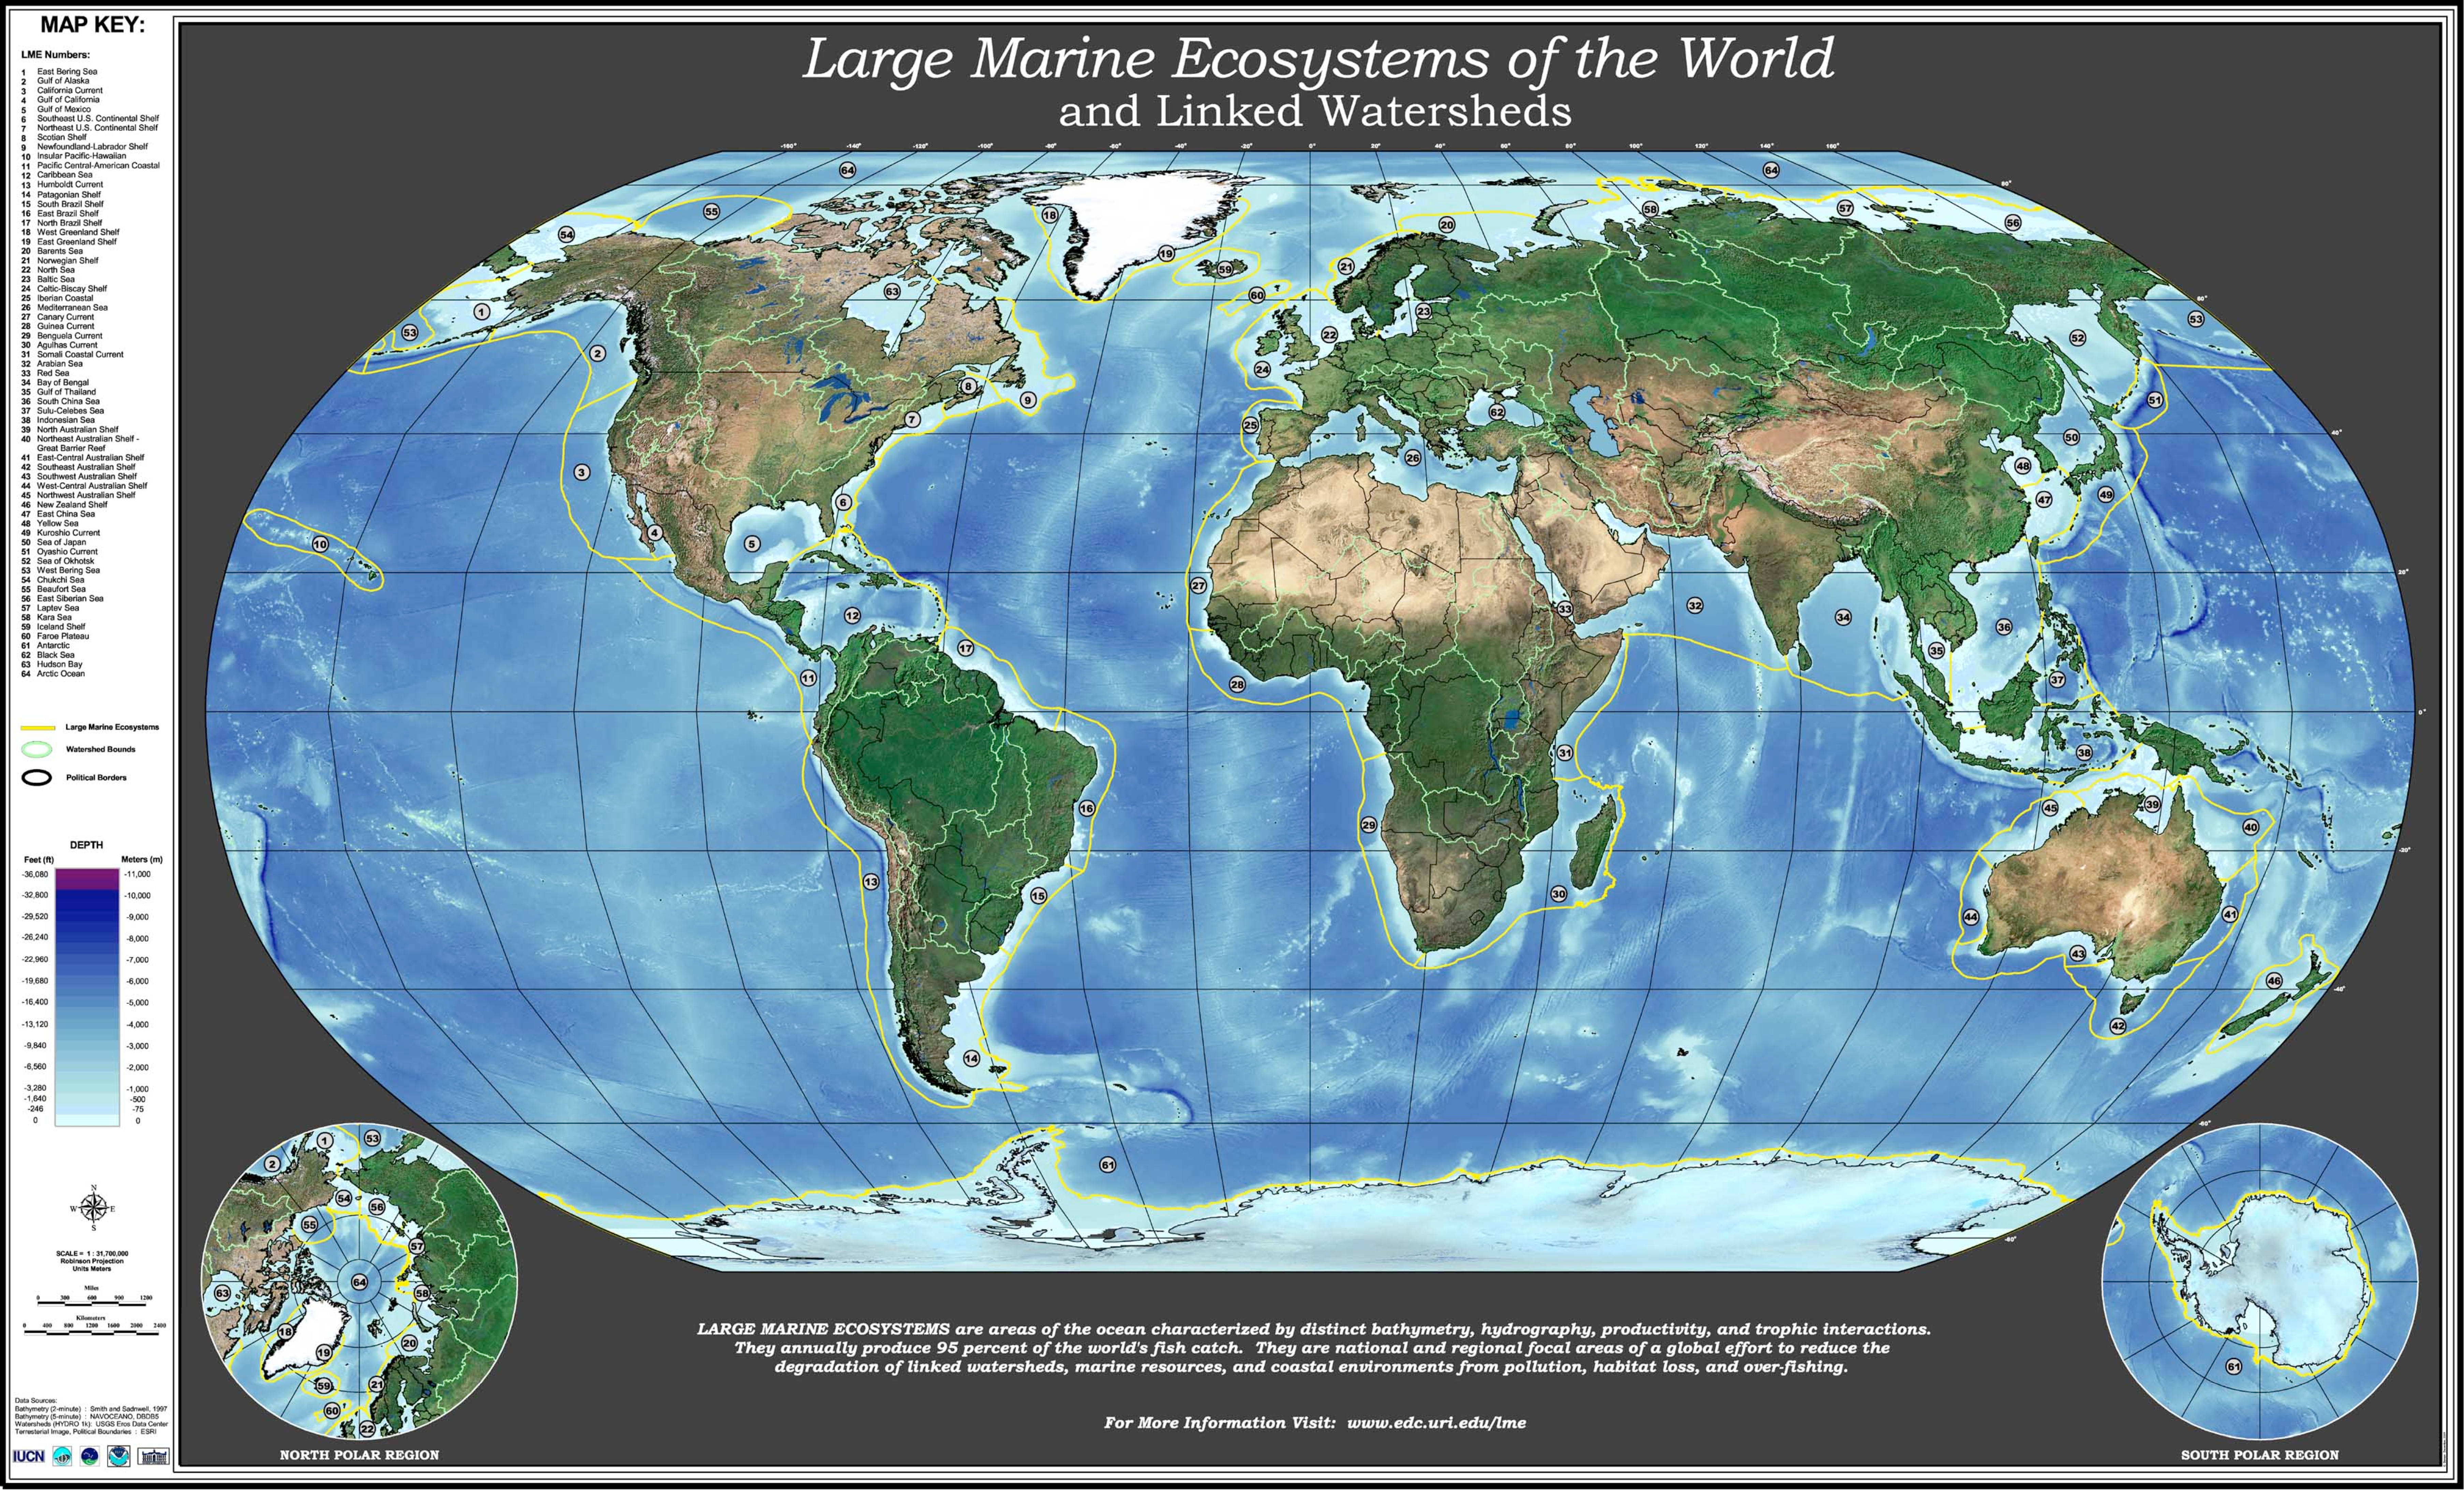
\includepdf[angle=90, addtotoc={1,subsubsection,1,LME map,lmemap}]{/home/srdbadmin/SQLpg/srdb/trunk/tex/lme_map.pdf}\end{document}
